\documentclass{tongjithesis}
\usepackage{tongjithesis}

%%%%%%%%%%%%%%%%%%%%%%%%%%%%%%%%%%%
% 若你想要用句点(.)替换句号(。)
% 可以打开下面的注释
%%%%%%%%%%%%%%%%%%%%%%%%%%%%%%%%%%%
% \catcode`\。=\active
% \newcommand{。}{\ifmmode\text{.}\else .\fi}
%%%%%%%%%%%%%%%%%%%%%%%%%%%%%%%%%%%

\begin{document}

\school{软件学院}
\major{软件工程}
\student{1953910}{李林洲}
\thesistitle{基于WebGPU的轻量级在线复杂流体仿真算法}{}
\thesistitleeng{Lightweight Online Complex Fluid Simulation Algorithm Using WebGPU}{}
\thesisadvisor{贾金原教授}
\thesisdate{2023}{06}{5}

\MakeCover


\pagestyle{firststyle}
\MakeAbstract{
    实时流体仿真是计算机图形学领域的重要研究课题,但在Web端进行流体仿真面临一系列挑战。传统的方法在追求稳定性的同时,往往牺牲计算效率,难以在性能有限的浏览器上实时运行。然而,WebGPU的出现为Web端流体仿真带来了新的机遇。作为一种新兴的图形渲染API,WebGPU通过全新的架构设计和接近底层硬件的接口,为图形应用提供了更高效的性能优化手段。本文旨在探索基于WebGPU的实时流体仿真方法,突破传统Web端流体仿真的困境,并为各个领域带来更便捷和强大的流体仿真工具。

    本文采用了一系列创新方法来实现基于WebGPU的实时流体仿真。首先,采用基于位置的流体模拟方法,通过迭代求解流体的密度约束,确保了模拟过程中流体的不可压缩性。其次,使用隐式边界条件表示方法来实现固液耦合,将固体边界对流体粒子的影响预计算到三维纹理中,提高了计算效率。第三,添加非压强力模型,包括表面张力、涡量补偿力和人工粘性力,以改善流体细节并提高模拟的真实感。第四,实现了完全并行化的高效邻近粒子搜索算法,通过空间网格划分和计算排序等技术加速搜索过程。最后,采用屏幕空间流体渲染方法,并设计了窄域滤波器用于深度图平滑,在重建流体表面的同时仍能够保留流体轮廓细节。

    通过多个复杂的流体仿真场景,本文验证了所提出方法的稳定性和高效性。实验结果表明,我们的流体仿真系统能够在性能有限的集成显卡上实现实时仿真,并达到30FPS以上的帧率。这证明了本文方法在计算效率方面的优越性和可行性,为Web端实时流体仿真提供了切实可行的解决方案。
}{WebGPU,实时流体仿真,平滑粒子流体动力学,基于位置的流体,屏幕空间渲染}

\MakeAbstractEng{
    Real-time fluid simulation is an important research topic in the field of computer graphics. However, conducting fluid simulation on the web faces a series of challenges. Traditional methods often sacrifice computational efficiency in pursuit of stability, making it difficult to achieve real-time performance on limited-performance browsers. However, WebGPU brings new opportunities for web-based fluid simulation. As an emerging graphics API, WebGPU provides more efficient performance optimization methods for graphics applications through a new architecture design and interfaces close to the underlying hardware. This paper aims to explore real-time fluid simulation methods based on WebGPU, overcome the limitations of traditional web-based fluid simulation, and provide more convenient and powerful fluid simulation tools for various fields.

    This paper adopts a series of innovative methods to achieve real-time fluid simulation based on WebGPU. Firstly, a position-based fluid simulation method is used to iteratively solve the density constraints of the fluid, ensuring the incompressibility of the fluid during the simulation process. Secondly, an implicit boundary representation method is used to realize solid-liquid coupling. The influence of solid boundaries on fluid particles is precomputed into a 3D texture, improving computational efficiency. Thirdly, non-pressure force models, including surface tension, vorticity confinement, and artificial viscosity, are added to improve fluid details and enhance simulation realism. Fourthly, a fully parallelized and efficient neighbor particle search algorithm is implemented, accelerating the search process through techniques such as spatial grid partitioning and counting sort. Finally, a screen-space fluid rendering method is employed, and a narrow-band filter is designed for depth map smoothing, allowing for the reconstruction of fluid surfaces while preserving fluid contour details.

    Through multiple complex fluid simulation scenarios, this paper validates the stability and efficiency of the proposed methods. Experimental results demonstrate that our fluid simulation system can achieve real-time simulation on integrated graphics processing unit of limited-performance, achieving frame rates of over 30 FPS. This demonstrates the superiority and feasibility of the proposed methods in terms of computational efficiency, providing a practical solution for real-time web-based fluid simulation.
}{WebGPU, Real-Time Fluid Simulation, SPH, PBF, Screen Space Rendering}


\clearpage
\tableofcontents   %放置目录
\clearpage

\pagestyle{mainstyle}
\section{引~言}
\subsection{背景介绍}
\subsubsection{WebGPU}
    如今,浏览器技术日新月异,大量Web APP提供的丰富内容远超“浏览网页”这种简单需求。根据他们的工作负载不同,可以将这些应用程序大致分为控制密集型(如搜索、解析、排序和网络请求)和数据密集型(如图像处理、数值计算、渲染和仿真)两种\cite{K22WebGPU1}。控制密集型应用往往在CPU上运行的更快,而高效地运行数据密集型应用则往往需要大规模并行计算架构处理器——GPU。一直以来,由于软硬件的限制,浏览器环境下并不善于处理大量数据计算。而近两年W3C提出的WebGPU图形API,为Web开发者提供了接近底层的GPU性能与大量现代的图形硬件特性,这使得在浏览器中运行更加富有创造力的应用——复杂流体仿真,成为了可能。
    
    WebGPU的设计目标之一是接替WebGL,这是自浏览器提供GPU支持以来最大规模的图形API架构变动。它给开发者提供了更加自由的硬件资源控制(如支持计算管线,开放通用计算功能), 与更科学的API设计(如指令队列,减少CPU与GPU通信)\cite{K22WebGPU2}。目前,多个3D引擎(Three.js、Babylon.js与Orillusion)都在积极推进对WebGPU的支持。

\subsubsection{实时流体仿真}
    实时流体仿真是计算机图形学领域一个重要的研究方向,涉及模拟流体行为的计算方法和技术。流体在许多领域中起着关键作用,包括游戏开发、动画制作、虚拟现实和工程仿真等。实时流体仿真的目标是以接近实时的速度模拟流体的运动、变形和相互作用,以便在交互式环境中提供逼真的视觉效果和物理反馈。
    
    传统的流体仿真方法通常基于数值求解或网格离散化的技术,如有限元方法或格点流体动力学。然而,这些方法在实时应用中的计算复杂度较高,难以满足实时性的要求。因此,研究者们正在不断探索更高效的实时流体仿真算法。
    
    其中一种被广泛应用的方法是基于粒子的平滑粒子动力学算法(Smoothed Particle Hydrodynamics,SPH)。SPH算法将流体系统离散化为一组粒子,并通过计算粒子之间的相互作用力来模拟流体的行为。SPH算法在处理流体的自由表面、非线性行为和复杂流动时表现出色。然而,由于涉及大量粒子之间的相互作用计算,SPH算法的实时性仍然是一个挑战。
    
    为了克服实时流体仿真的挑战,研究者们开始利用现代计算技术,如图形处理器(GPU)和并行计算,来加速流体仿真算法。而WebGPU正是提供了高性能的并行计算和图形渲染能力。通过结合SPH算法和WebGPU技术,可以实现轻量级的在线复杂流体仿真,使得流体仿真能够在Web浏览器中以接近实时的速度进行。
    
    因此,本毕业设计旨在研究基于WebGPU的轻量级实时流体仿真算法,特别关注SPH算法在Web平台上的加速和优化。通过使用WebGPU的并行计算和高性能图形渲染能力,预计可以改善实时流体仿真的性能和交互性,从而推动在线流体仿真应用的发展。这项研究对于提升实时流体仿真技术的效率和实用性具有重要意义。

\subsection{本文主要工作}
    本文的主要目标是使用WebGPU实现一个轻量级在线3D复杂流体仿真系统,主要工作概况为以下三点:

    \begin{enumerate}
    	\item 设计了一套流体模拟算法。本文使用粒子法的作为流体模拟的主要框架。为了保证不可压缩性,本文使用基于位置的动力学思想迭代求解密度约束,并使用一种隐式边界表示方法——边界体积贴图法实现流体固液耦合。另外,为了进一步提高流体模拟真实感,本文在流体压强求解器之后又加入了三种非压强力的求解模型——表面张力、涡量补偿力与人工粘性力。最后,本文实现了通过空间划分加速的邻域粒子查找算法。
    	\item 设计了一套流体渲染算法。针对粒子法流体仿真的结果,本文提出了一种高效的流体渲染方案。首先将粒子光栅化得到深度图和厚度图,再对深图进行窄域滤波,最后进行屏幕空间渲染。
    	\item 使用WebGPU实现了流体仿真系统。本文将模拟与渲染算法完全并行化,使用WebGPU实现。本仿真系统可以实时运行十万个流体粒子的仿真规模,并完成实时高质量渲染。经过多个仿真场景的实际检验,可以证明仿真系统达到了设计目标。
    \end{enumerate}

\subsection{本文组织结构}
    本文共有八个章节,本文主要介绍了WebGPU与实时流体仿真的相关背景,并简要概括了本文的主要工作。本文后续章节概要如下:
    
    第二章详细介绍了流体模拟的当前研究现状与工作总结,包括粒子法、网格法以及粒子-网格混合法。
    
    第三章将详细介绍基于位置的不可压缩流体的密度约束求解算法,以及边界体积贴图这种隐式边界条件算法。
    
    第四章将介绍用于改善流体细节的三种非压强力,它们分别是表面张力、涡量补偿力与人工粘性力。
    
    第五章将介绍基于空间网格划分的邻域粒子并行查找算法,其中又进一步介绍了数组前缀和并行计算方法及其GPU实现优化细节。
    
    第六章将介绍流体屏幕空间渲染算法,用于将流体粒子实时渲染。
    
    第七章详细介绍了WebGPU架构与重要API功能,然后阐述了流体仿真系统的算法实现方案,最后构建多个实际场景证明系统的可靠性。
    
    第八章总结全文介绍的算法与工作,并分析了本文仿真框架存在的不足与限制,最后展望了浏览器端实时流体仿真的广阔应用前景。
\clearpage
\section{相关工作}
\subsection{纳维斯托克方程}

    流体在生活中无处不在,比如水、烟雾、火焰等等,它们的运动复杂多样,所以通过计算机模拟流体运动的呈现的视觉效果是图形学重要的一部分。目前,流体仿真越来越广泛地应用于工程模拟、游戏开发、虚拟现实等领域。在物理上,不可压缩流体的运动可以用一组偏微分方程所描述,即纳维-斯托克斯方程(Navier-Stokes Equations)\cite{BM07Fluid, B15Fluid}:

    \begin{equation}\label{eq:ns1}
    	\frac{\partial \mathbf{u}}{\partial t} = -\mathbf{u} \cdot \nabla \mathbf{u} - \frac {1}{\rho} \nabla p + \mathbf{g} + \mu \nabla \cdot \nabla \mathbf{u}
    \end{equation}
    
    \begin{equation}\label{eq:ns2}
    	\nabla \cdot \mathbf{u} = 0
    \end{equation}

    其中,$\mathbf{u}$ 为速度,$\rho$ 为密度,$p$ 为压强,$\mu$ 为粘滞系数, $\mathbf{g}$ 为重力加速度。公式\ref{eq:ns1}描述了动量守恒,流体速度场的变化受四个因素的影响,分别是:速度本身导致的变化,压强,外力与粘滞力。而公式\ref{eq:ns2}则描述了质量守恒,即流体是不可压缩的,所以速度场的散度为零。因此,如何离散化求解N-S方程就是流体模拟的关键所在,而不同的模拟方法可以根据离散化的视角不同划分为三类:欧拉视角(网格法),拉格朗日视角(粒子法)以及混合欧拉-拉格朗日视角(网格-粒子混合方法)。

    在欧拉视角下,流体所在的空间被划分为均匀网格,网格自身的位置并不随流体的运动而改变。同时,在每个格点上存储物理量,如速度、压强、浓度等。显然,均匀网格可以使得计算时很容易随机访问物理量。但是,难以计算流体运动给网格上的物理量带来的变化。代表方法如Stable Fluids\cite{FSJ01Somke, S99EM}。

    在拉格朗日视角下,流体自身被离散化为大量粒子,粒子随着流体一起运动,在每个粒子上存储物理量,如位置,速度,质量等。显然,自由的粒子可以方便地模拟流体的运动,只需要改变粒子的位置即可。但是,这种方法难以计算粒子之间的互相影响,因为不能直接访问某位置附近的粒子。代表方法如平滑粒子流体动力学(Smoothed Particle Hydrodynamics, SPH)\cite{M92SPH}。

    而混合欧拉-拉格朗日视角相当于结合了前两者,空间中即存在网格也存在粒子。先后在粒子和网格上计算相对容易的部分,通过插值方法将物理量在粒子和网格上相互转换。显然,这种方法使前两个方法取长补短,但是物理量在粒子和网格之间的转换又会造成不必要的时间和空间开销。代表方法有:PIC(Particle in Cell)\cite{H62PIC}、FLIP(Fluid Implicit Particles)\cite{BR86FLIP}、物质点法(Material Point Method,MPM)\cite{JST16MPM}。

\subsection{基于网格的模拟方法}

    欧拉法是通过均匀网格离散空间物理场的流体模拟方法。Harlow和Welch\cite{HW65MAC}提出了MAC(Marker-and-cell)网格,将速度的xyz分量分别保存在网格的面上而非网格中心,这样做提高了差分计算的数值精度,并且避免了非平凡零空间问题。欧拉法的算法步骤可以分为:平流(Advection),添加外力(Body force),扩散(Diffusion)和压强投影(Pressure projection)。

    平流是欧拉法流体模拟的一个关键步骤,因为网格法描述流体移动不像粒子法一样简单,所以平流步骤的准确程度对模拟效果有很大影响。最简单的Advection方案是semi-Lagrangian法,即以当前格点 $x_1$ 位置的速度向后推一个时间步长,得到 $x_2$ 位置,认为 $x_1$ 位置的流体由 $x_2$ 流动而来,其物理量也可以由 $x_2$ 位置插值得到。这种方法可以用龙格库塔法(Runge-Kutta)将时间步分成多段计算,进一步提高数值精度。Kim\cite{KLL06BFECC}等人提出了BFECC方法,该方法执行多个向后和向前Advection步骤,以纠正空间和时间误差。Jonas\cite{ZNT18AR}等人进一步提出了在模拟步骤中间应用反射算子,大大降低了能量耗散。

    计算外力是几个较为简单的步骤,一般只有重力,而在模拟烟雾等气体是,需要考虑温度场和密度场变化所带来的浮力,在\textit{Fluid Engine Development}一书中有具体实现\cite{K17Fluid}。

    流体扩散即计算粘滞力,对应这公式\ref{eq:ns1}的最后一项,其由速度的拉普拉斯表示。具体实现可以分为前向欧拉积分和后向欧拉积分,前向欧拉积分实现简单,但是对大时间步长不稳定,后向欧拉积分需要求解一个全局的稀疏线性系统,但是可以稳定模拟。由于Advection步骤中的插值运算会带来“数值粘性”,如果模拟水这种粘性较小的液体,可以不计算流体扩散。
    
    压强投影是欧拉法流体模拟的关键,正确地计算压强,才能保证速度场无散,流体不可压缩。压强投影的步骤如下:首先计算速度场散度,然后求解压强泊松方程,最后通过压强梯度得到无散速度场。求解泊松方程的常用方法有雅可比迭代法,高斯-塞德尔迭代法,而最高效的解算器是预条件共轭梯度法(Preconditioned Conjugate Gradient, PCG)\cite{HK12IPPCG}。常用的PCG方法有ICPCG(Incomplete Cholesky PCG)、IPPCG(Incomplete Poisson PCG)\cite{HK12IPPCG}以及MGPCG(Multigrid PCG)\cite{MST10MGPCG}。
    
    压强投影的迭代计算是欧拉法流体模拟的性能瓶颈。Frank\cite{LGF04EM}等人使用八叉树优化网格数据结构。Stam\cite{S03EM}进一步简化Stable Fluids方法使得其能实时运行。Harris\cite{H05EM}使用GPU加速流体模拟。Rabbani\cite{RGR22CPF}又提出了使用两次可分离滤波比较精确地近似迭代法压力投影计算,在提高性能的同时,保证模拟的结果。

\subsection{基于粒子的模拟方法}

    SPH是拉格朗日视角流体模拟的代表方法,它源自天体物理学领域\cite{M92SPH, CR99SPH},Müller\cite{MCG03SPH}等人将此方法首先用于计算机图形学流体模拟。SPH是一种基于积分插值理论的方法,它通过自由移动的粒子来作为空间中连续物理场的离散采样点,空间中任意位置的物理量或微分值可以由临近粒子的值加权平均得到。

    \begin{equation}
    	A_i = \sum_j \frac {m_j} {p_j} A_j w_{ij}
    \end{equation}
    
    其中 $A$ 为插值物理量,$m$ 为粒子质量,$w$ 为核函数插值权重。具体的核函数有多种,如Poly6,Spiky等\cite{MCG03SPH}。在确定好如何离散化空间之后,可以得出SPH的基本算法框架:首先计算所以粒子的密度,其次计算粘滞力与外力,然后求解压强,最后根据时间步更新粒子速度与位置。与欧拉法模拟一样,最关键的步骤在于压强求解。而求解压强又可以分为两类方法,一种是EOS(Equation Of State),另一种是PPE(Pressure Poisson Equation)\cite{KBS19SPH}。
    
    EOS是一种局部的压强解算方法,它计算粒子与其邻近粒子的密度差,通过状态方程将其转化为此粒子处的压强。也就是说在流体被压缩或膨胀后计算出恢复原状的作用力,所以这种方法模拟的流体是可压缩或弱可压缩的,如WCSPH(Weakly Compressible SPH)\cite{BT07WCSPH}。这种方法实现简单,可以对每个粒子独立地计算压强而不用解一个全局的线性系统。但是这种方法模拟的可压流体效果一般,且需要较小的时间步长。
    
    PPE是一种全局的压强解算方法。它往往采样了迭代式的算法框架,从而保证流体的不可压缩性。四个当前主流的PPE压强结算方法为:IISPH(Implicit Incompressible SPH)\cite{ICS13IISPH}、PCISPH(Predictive-corrective Incompressible SPH)\cite{SP09PCISPH, BET10PCISPH}、PBF(Position Based Fluid)\cite{MM13PBF}和DFSPH(Divergence-free SPH)\cite{BK15DFSPH, BK16DFSPH}。Dan等人在SPH综述\cite{KBS22SPH}中证明了这几种算法的等价性。
    
    SPH最大的算法瓶颈在于邻近粒子搜索,如果不做任何优化,邻居搜索的时间复杂度为 $O(n^2)$,这显然是不能接受的。Green\cite{G10NS}给出了基于Cuda的邻居搜索优化方案:在空间中建立间隔为搜索半径的均匀网格,将粒子放在网格中,搜索时只需查找27个网格中的粒子即可。但是三维空间会大大消耗存储空间,所以Ihmsen\cite{IAB11NS}等人提出了紧凑哈希(Compact Hashing)算法,使用哈希表压缩三维网格,同时使用Z-curve进行排序,以保证空间局部性,提高缓存命中率。

\subsection{网格-粒子混合模拟方法}

    PIC是最原始的混合欧拉-拉格朗日方法,它在网格上计算压强投影,而使用粒子完成Advection。FLIP\cite{ZB05FLIP}通过“隐式粒子”改善了PIC的数值耗散问题,但是却降低了模拟的稳定性。APIC(Affine Particle in Cell)\cite{JSS15APIC, JST17APIC}通过引入仿射变换来计算粒子的速度,提高精度的同时保证了角动量守恒。
    
    MPM\cite{JST16MPM}方法则可以模拟范围更广的物理材质,如弹塑性物体。MLS-MPM(Moving Least Square MPM)\cite{HFG18MSLMPM, HLA19Taichi}大大改进了MPM的计算效率。与PIC或FLIP方法不同,MPM方法更接近于拉格朗日法,它并不在网格上求解压强投影,网格更像是一种加速粒子相邻区域插值的辅助结构。所以模拟时往往需要较小的时间步长。

\subsection{流体渲染}

    与流体模拟相同,流体渲染的方法也多种多样,一方面,针对离线应用或实时应用的渲染方法不同,另一方面,针对不同的模拟方法(网格法/粒子法),所采取的渲染方法也不尽相同。由于网格和粒子都可以看作对空间中流体的采样,所以在恢复流体表面时,如何既能使得表面平滑,又能保留流体的细节(如水花、波浪等),是各种流体渲染方法都需要面临的挑战。
    
    其中一个主流的方法是重建流体表面。在网格模拟方法中,流体表面就是水平集(Level Set)\cite{OS88LS}为0的隐式表面。由于空间已经被划分为均匀网格,可以直接在这个网格上使用经典的移动立方体\cite{LC87MC}(Marching Cubes)算法。相比之下,粒子模拟方法就需要通过每个粒子的核函数相互重叠来定义标量密度场,然后在这个标量场中使用移动立方体方法提取等值面。Jihun\cite{YT13AK}等人提出使用主成分分析得到各向异性的核函数,从而使得重建表面更加平滑。如果需要高质量的重建结果,Akinci等人建议使用粒子间距一半的网格密度重建表面\cite{AIA12SR, AAI12SR}。显然这种方法一般只能用于离线应用。另外也有一些不重建表面的方法,例如,随着模拟时间推移而优化显示网格的表面追踪方法\cite{EFF02LS},通过元球\cite{KSN08MB, ZSP08ASR}(Metaballs)或距离场\cite{GSS10SPH}计算光线和等值面的交点从而避免多边形化。
    
    如果需要实时渲染,屏幕空间的渲染方法就是一个不错的解决方案。这些方法有一个共性,它们都从球型粒子光栅化得到深度图,再对深度图进行平滑,最后在屏幕空间渲染。由于大部分计算都在2D完成,所以这些方法非常高效。在PBD中,深度图经过二项式滤波器,再使用移动正方形提取对相机可见的粒子\cite{MHH07PBD}。相比之下,一些方法\cite{VGS09SSF, G10SSF, BSW10LPF, TY18NRSSF}可以直接将深度图用于最终渲染。Van\cite{VGS09SSF}等人平滑了粒子间的曲率变化。Bagar\cite{BSW10LPF}等人进一步拓展了此方法,使得平滑程度与相机距离无关。与平滑曲率不同,Green\cite{G10SSF}使用高斯滤波平滑深度图,并使用双边权重来保持轮廓边缘。如果将2D滤波器替换为两个方向的1D滤波器,计算效率会大大提升,但同时带来一些可接受的伪影状瑕疵。Truong\cite{TY18NRSSF}等人提出了一种窄幅滤波器,提高了平滑效果的同时保留了流体边缘的清晰轮廓。同时,他们发现如果在两个方向的1D滤波之后再进行一遍半径很小的2D滤波,由于滤波器的不可分离性带来的伪影状瑕疵会大大减轻。
    
    另外,Akinic\cite{ADA13SSF}等人提出了一种在屏幕空间渲染水花泡沫的方法。Imai\cite{IKM16SSF}等人提出了实时渲染液体复杂折射的方法,从而提高流体渲染的真实感。
\clearpage
\section{实时流体模拟算法}
    流体的运动千变万化,通过计算机模拟流体的运动状态是图形学中一个重要的研究课题,它广泛应用于影视、广告、游戏等领域。为了表现复杂灵动的流体,往往需要消耗大量的计算资源,所以实时流体模拟比离线方法更加困难。本文采用了平滑粒子动力学方法进行实时流体模拟,而本章主要阐述了其中压强求解的算法框架,这是保证流体仿真高效、稳定、真实的重要因素。

    \begin{figure}[htbp]
    	\centering
    	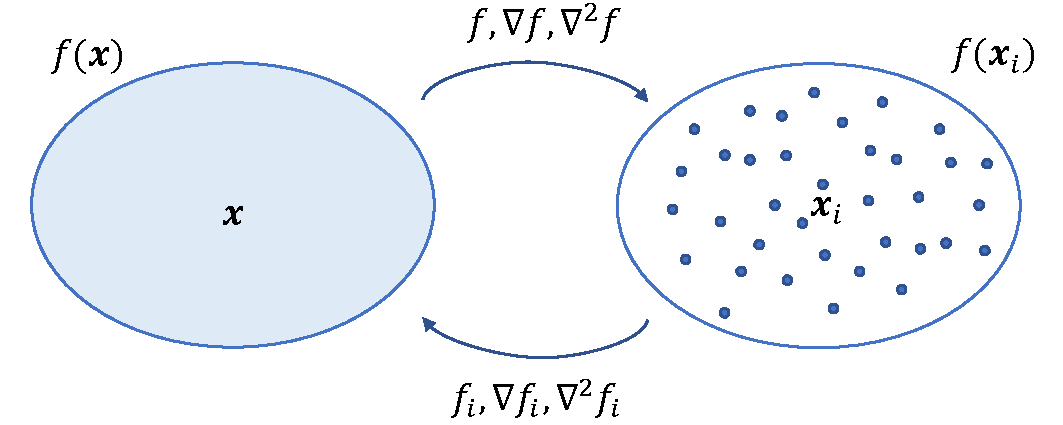
\includegraphics[width=.7\textwidth]{figures/simulation/field.pdf}
    	\caption{SPH物理场离散}
    \end{figure}

\subsection{平滑粒子动力学}
    在宏观尺度的视角下,现实世界的物理现象在空间和时间上都是连续的,为了在计算机上模拟这些现象,首要解决的问题是如何离散这些物理量。在时间上,往往会选择划分为一个个微小时间步,通过显式或隐式时间积分来体现流体的运动。在空间上,可以选择将空间划分为网格或者粒子,它们的区别是网格位置在模拟过程中是不变的,而粒子会随着流体的运动而改变位置。由于粒子之间没有连接关系,所以粒子法比网格法更灵活,更适用于自由表面流体的模拟。

    平滑粒子动力学(SPH)是粒子法的一种,将物理场离散为粒子之后,它通过核函数对离散点积分求得任意位置物理量的近似值(如图\ref{fig:kernelfunc}),而梯度值也可以由核函数梯度积分得到。
    \begin{equation}
    	\begin{gathered}
    	f(\mathbf{x}_i) = \sum_j \frac{m_j}{\rho_j} f(\mathbf{x}_j) W(\mathbf{x}_i - \mathbf{x}_j)
    	\\
    	\nabla f(\mathbf{x}_i) = \sum_j \frac{m_j}{\rho_j} f(\mathbf{x}_j) \nabla W(\mathbf{x}_i - \mathbf{x}_j)
    	\end{gathered}
    \end{equation}
    当 $f$ 为粒子密度时,可以得到流体密度的计算公式
    \begin{equation}\label{eq:densfunc}
    	\rho_i = \sum_j m_j W(\mathbf{x}_i - \mathbf{x}_j)
    \end{equation}
    核函数的定义有许多种,但需要满足以下五个条件:
    \begin{enumerate}
    	\item 归一化条件:$\int_{\mathbb{R}^d} W(\mathbf r, h)\,\mathrm d v = 1$
    	\item 狄拉克$\delta$条件:$\lim_{h\rightarrow 0} W(\mathbf r, h) = \delta (\mathbf r)$
    	\item 非负性条件:$W(\mathbf r, h) \ge 0$
    	\item 对称性条件:$W(\mathbf r, h) = W(\mathbf r, h)$
    	\item 紧支撑条件:$W(\mathbf r, h) = 0 \quad \mathrm{for}\; |\mathbf r| > h$
    \end{enumerate}
    本文中,我们使用Poly6核函数计算一般物理量,而使用Spiky核函数计算物理量梯度\cite{MCG03SPH},定义如下
    \begin{equation}
    	\begin{gathered}
    	W_{\mathrm{Poly6}}(\mathbf r, h) = \frac{315}{64 \pi h^9}
    	\left\{
    	\begin{array}{ll}
    	(h^2 - |\mathbf r|^2)^3 & 0 \le |\mathbf r| < h \\
    	0 & \mathrm{otherwise} \\
    	\end{array}
    	\right.
    	\\
    	\nabla W_{\mathrm{Spiky}}(\mathbf r, h) = -\frac{45}{\pi h^6}
    	\left\{
    	\begin{array}{ll}
    	\frac{\mathbf r}{|\mathbf r|} (h - |\mathbf r|)^2 & 0 < |\mathbf r| < h \\
    	\mathbf 0 & \mathrm{otherwise} \\
    	\end{array}
    	\right.
    	\end{gathered}
    \end{equation}
    其中 $h$ 为核函数支撑域半径,$\mathbf r$ 为采样点到核函数中心的方向向量。
    
    \begin{figure}
    	\centering
    	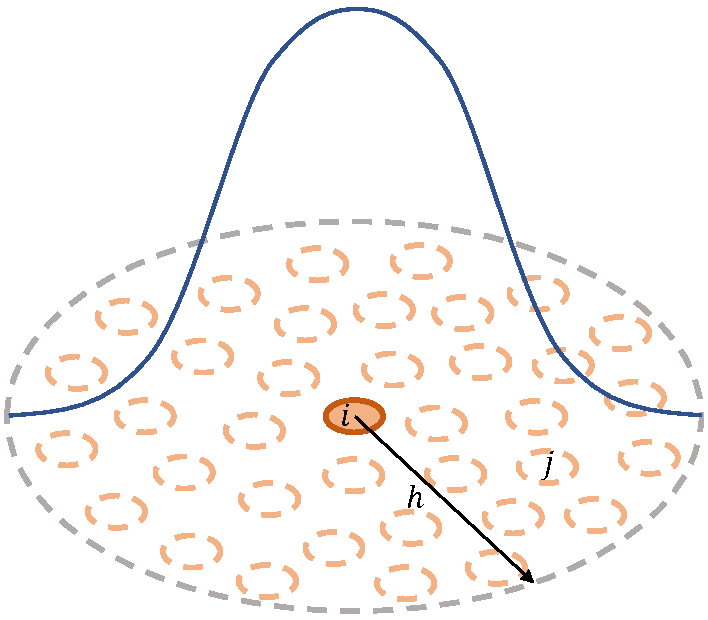
\includegraphics[width=.45\textwidth]{figures/simulation/kernel.pdf}
    	\caption{平滑核估计}
    	\label{fig:kernelfunc}
    \end{figure}
    
    \begin{figure}
    	\centering
    	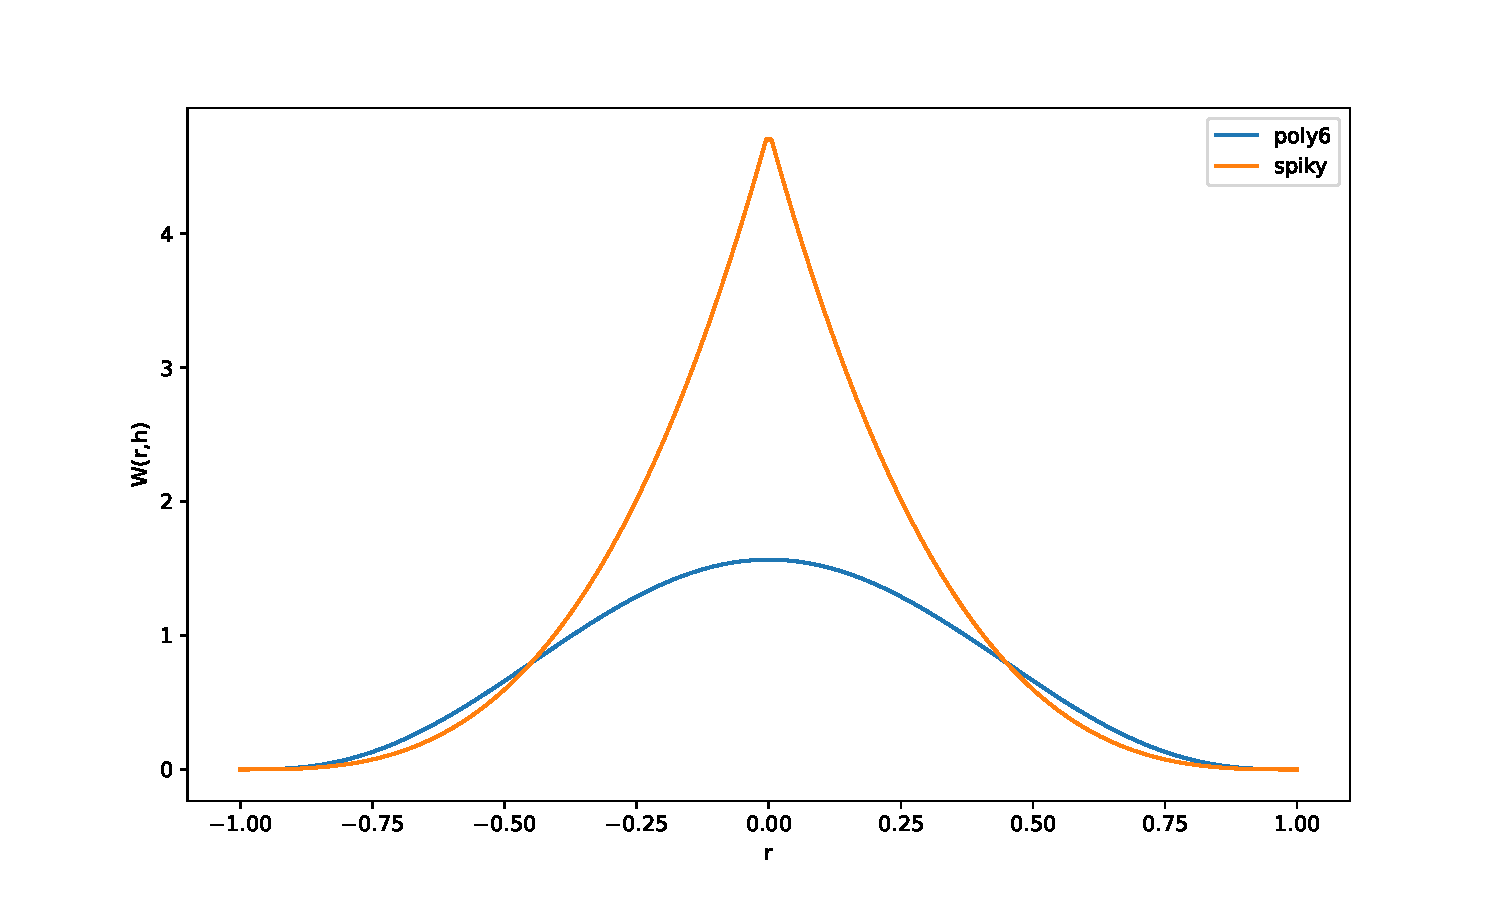
\includegraphics[width=.85\textwidth]{figures/simulation/kernel_func.pdf}
    	\caption{核函数示意图}
    \end{figure}

\subsection{基于位置的流体}
    在表现流体运动状态时,保证不可压缩性是体现流体真实感的关键因素。而不可压缩性在物理上可以描述为速度场旋度为0($\nabla \cdot \mathbf v = 0$),或密度场恒定($\rho = \rho_0$ )。大部分图形学中的模拟方法都是通过这两个条件之一计算流体压强与受力,再通过牛顿第二定律计算加速度,最后通过时间积分得到粒子速度与位置。而Macklin等人\cite{MM13PBF}提出了基于位置的方法(PBF),将不可压缩性条件转化为粒子位置约束,忽略了繁琐的时间积分过程,直接更新粒子位置。这种方法更加高效且容易控制。

\subsubsection{强制不可压缩约束}
    为了满足流体密度恒定的条件,我们需要求解一个非线性的约束 $\mathbf C$,且在每个流体粒子上都存在一个约束 $C_i$。每个约束都可以写成粒子位置及其近邻粒子位置的函数,根据密度计算公式\ref{eq:densfunc},我们可以将第 $i$ 个粒子的约束状态表示为
    \begin{equation}
    	C_i(\mathbf{x}_1,...,\mathbf{x}_n)  = \frac {\rho_i} {\rho_0} - 1
    \end{equation}
    其中 $\rho_0$ 为初始状态流体密度。我们的求解目标是对每个粒子寻找一个位置更新向量 $\Delta \mathbf x_i$,使得所有约束条件都满足 $C_i(\mathbf x + \Delta \mathbf x_i) = 0$。那么对于整个约束系统就意味着
    \begin{equation}\label{eq:constrainsys}
    	\mathbf C(\mathbf x + \Delta \mathbf x) = \mathbf 0
    \end{equation}
    这个非线性约系统显然难以直接求解,所以我们使用牛顿法迭代优化的思想,每次迭代沿着位置约束函数的梯度方向更新位置,设更新步长为 $\lambda$,则
    \begin{equation}
    	\Delta \mathbf x = \nabla \mathbf C(x) \lambda
    \end{equation}
    进一步对公式\ref{eq:constrainsys}进行泰勒展开,可以得到:
    \begin{equation}
    	\begin{aligned}
    	\mathbf C(\mathbf x + \Delta \mathbf x) 
    	& \approx \mathbf C (\mathbf x) + \nabla \mathbf C^T(\mathbf x) \Delta \mathbf x \\
    	& \approx \mathbf C (\mathbf x) + \nabla \mathbf C^T(\mathbf x) \nabla \mathbf C(\mathbf x) \lambda = 0 \\
    	\end{aligned}
    \end{equation}
    在泰勒展开后忽略高阶项,我们的目标是使得约束为零,则可以利用这个条件反过来求得更新步长
    \begin{equation}\label{eq:lambda1}
    	\begin{gathered}
    	\lambda = - \frac {\mathbf C (\mathbf x)} {\nabla \mathbf C^T(\mathbf x) \nabla \mathbf C(\mathbf x)} \\
    	\lambda_i = - \frac {C_i} {\sum_k |\nabla_k C_i|^2}
    	\end{gathered}
    \end{equation}


\subsubsection{更新步长与位置更新向量}
    上文推导了PBF是如何迭代求解约束系统(公式\ref{eq:constrainsys})的,接下来我们需要具体推导每次迭代中更新步长和位置更新向量的计算公式。

    第一节公式\ref{eq:ns1}介绍了如何SPH方法如何计算物理场及其梯度,我们可以按照同样的方法计算约束函数的梯度。具体地,约束 $C_i$ 对粒子 $k$ 梯度如下式所示,需要注意的是,某粒子对应的约束对其本身球梯度或是对其近邻粒子求梯度,计算公式是不同的。
    \begin{equation}
    	\begin{aligned}
    	\nabla_k C_i &= \frac {1} {\rho_0} \sum_j m_j \nabla_k W_{ij} \\
    	&=
    	\frac {1} {\rho_0}
    	\left\{
    	\begin{array}{ll}
    	\sum_j m_j \nabla W_{ij} & \mathrm{if} \ k = i \\
    	-m_j \nabla W_{ij} & \mathrm{if} \ k = j \\
    	\end{array}
    	\right.
    	\\
    	\end{aligned}
    \end{equation}
    将其代入公式\ref{eq:lambda1},可得 $\lambda_i$ 的具体计算公式为
    \begin{equation}\label{eq:lambda2}
    	\lambda_i = - \frac 
    	{ \max(\frac{\rho_i} {\rho_0} - 1, 0) } 
    	{ \frac {1}{\rho_0^2} (|\sum_j m_j \nabla W_{ij}|^2 + \sum_j |m_j \nabla W_{ij}|^2 ) + \varepsilon }
    \end{equation}
    
    由于公式\ref{eq:constrainsys}是非线性的,并且在核函数逼近其边界时梯度非常小,所以公式\ref{eq:lambda1}的分母会在粒子间距逼近核函数半径时造成整个系统的不稳定。因此我们在公式\ref{eq:lambda2}的分母中引入松弛参数 $\varepsilon$ 防止计算崩溃。这相当于正则化约束函数,即
    \begin{equation}
    	\mathbf C(\mathbf x + \Delta \mathbf x) 
    	\approx \mathbf C (\mathbf x) + \nabla \mathbf C^T(\mathbf x) \nabla \mathbf C(\mathbf x) \lambda + \varepsilon \lambda = 0
    \end{equation}

    最后,在得到更新步长之后,可以计算位置更新向量
    \begin{equation}
    	\Delta \mathbf x_i = \lambda_i \nabla_iC_i = 2\lambda_i \frac{1}{2\rho_0} \sum_j m_j \nabla W_{ij} \approx
    	\frac{1}{2\rho_0} \sum_j (m_i \lambda_i + m_j \lambda_j) \nabla W_{ij}
    \end{equation}
    
    SPH流体模拟通常会由于粒子没有足够的临近粒子,局部无法满足密度恒定约束从而产生负压强,导致粒子过度聚集。Macklin等人引入了人工压强项\cite{M00SPH}防止这一现象,同时模拟了表面张力效果。不过这并不是物理正确的,需要调整参数在缓解粒子聚集和表面张力效果之间寻找一个平衡点。而本文中直接不考虑负压强的影响(公式ref{eq:lambda2}分子),同时在仿真框架中引入表面张力模型,计算物理正确的粒子间内聚力与表面张力。表面张力建模将在第四章中详细阐述。

\subsection{边界条件}

    上文描述了流体粒子之间的运动状态求解,但是流体不可能在一个无限的空间中运动,所以需要确定流体粒子如何与固体边界进行交互。本节仅考虑流体与固体单向耦合,即固体是静态的,不会由于流体碰撞而发生移动。PBF框架是完全基于位置计算密度约束的,所以可以直接改变粒子位置使其满足边界条件,即在更新粒子位置时判断其是否超出了边界范围,如果超出边界则直接将其位置改变至边界内部。
    
    这种方法简单有效,但不是物理正确的,这会导致边界处粒子欠采样,而为了满足密度约束,会有大量粒子聚集在边界附近。一种常用的解决方法是将固体边界也离散化为粒子\cite{AIA12SPHB},将固体粒子也参与到流体粒子的密度计算和压强计算中来。但是这种方法消耗存储空间较大,且边界越复杂固体粒子越多需要离散的精度也越高。由于浏览器端资源空间受限,本文所实现的流体仿真框架所支持的最高粒子数为256k(详见5.3.4节), 使用固体粒子的方法虽然简单但是会大大压缩流体粒子的数量,降低流体仿真的真实感。所以本文采用Bender等人\cite{BKW19SPHB}提出的边界体积贴图(Volume Map)方法,这是一种隐式的边界表示方法,需要预计算空间每处边界固体的体积,而后在实时仿真中就可以通过贴图的方式高效查找。在原理上,体积贴图(Density Map)\cite{KB17SPHB}是密度贴图的改进方法,所以本文将先介绍密度贴图方法,再介绍体积贴图的改进点与具体实现。
    
    \begin{figure}
    	\centering
    	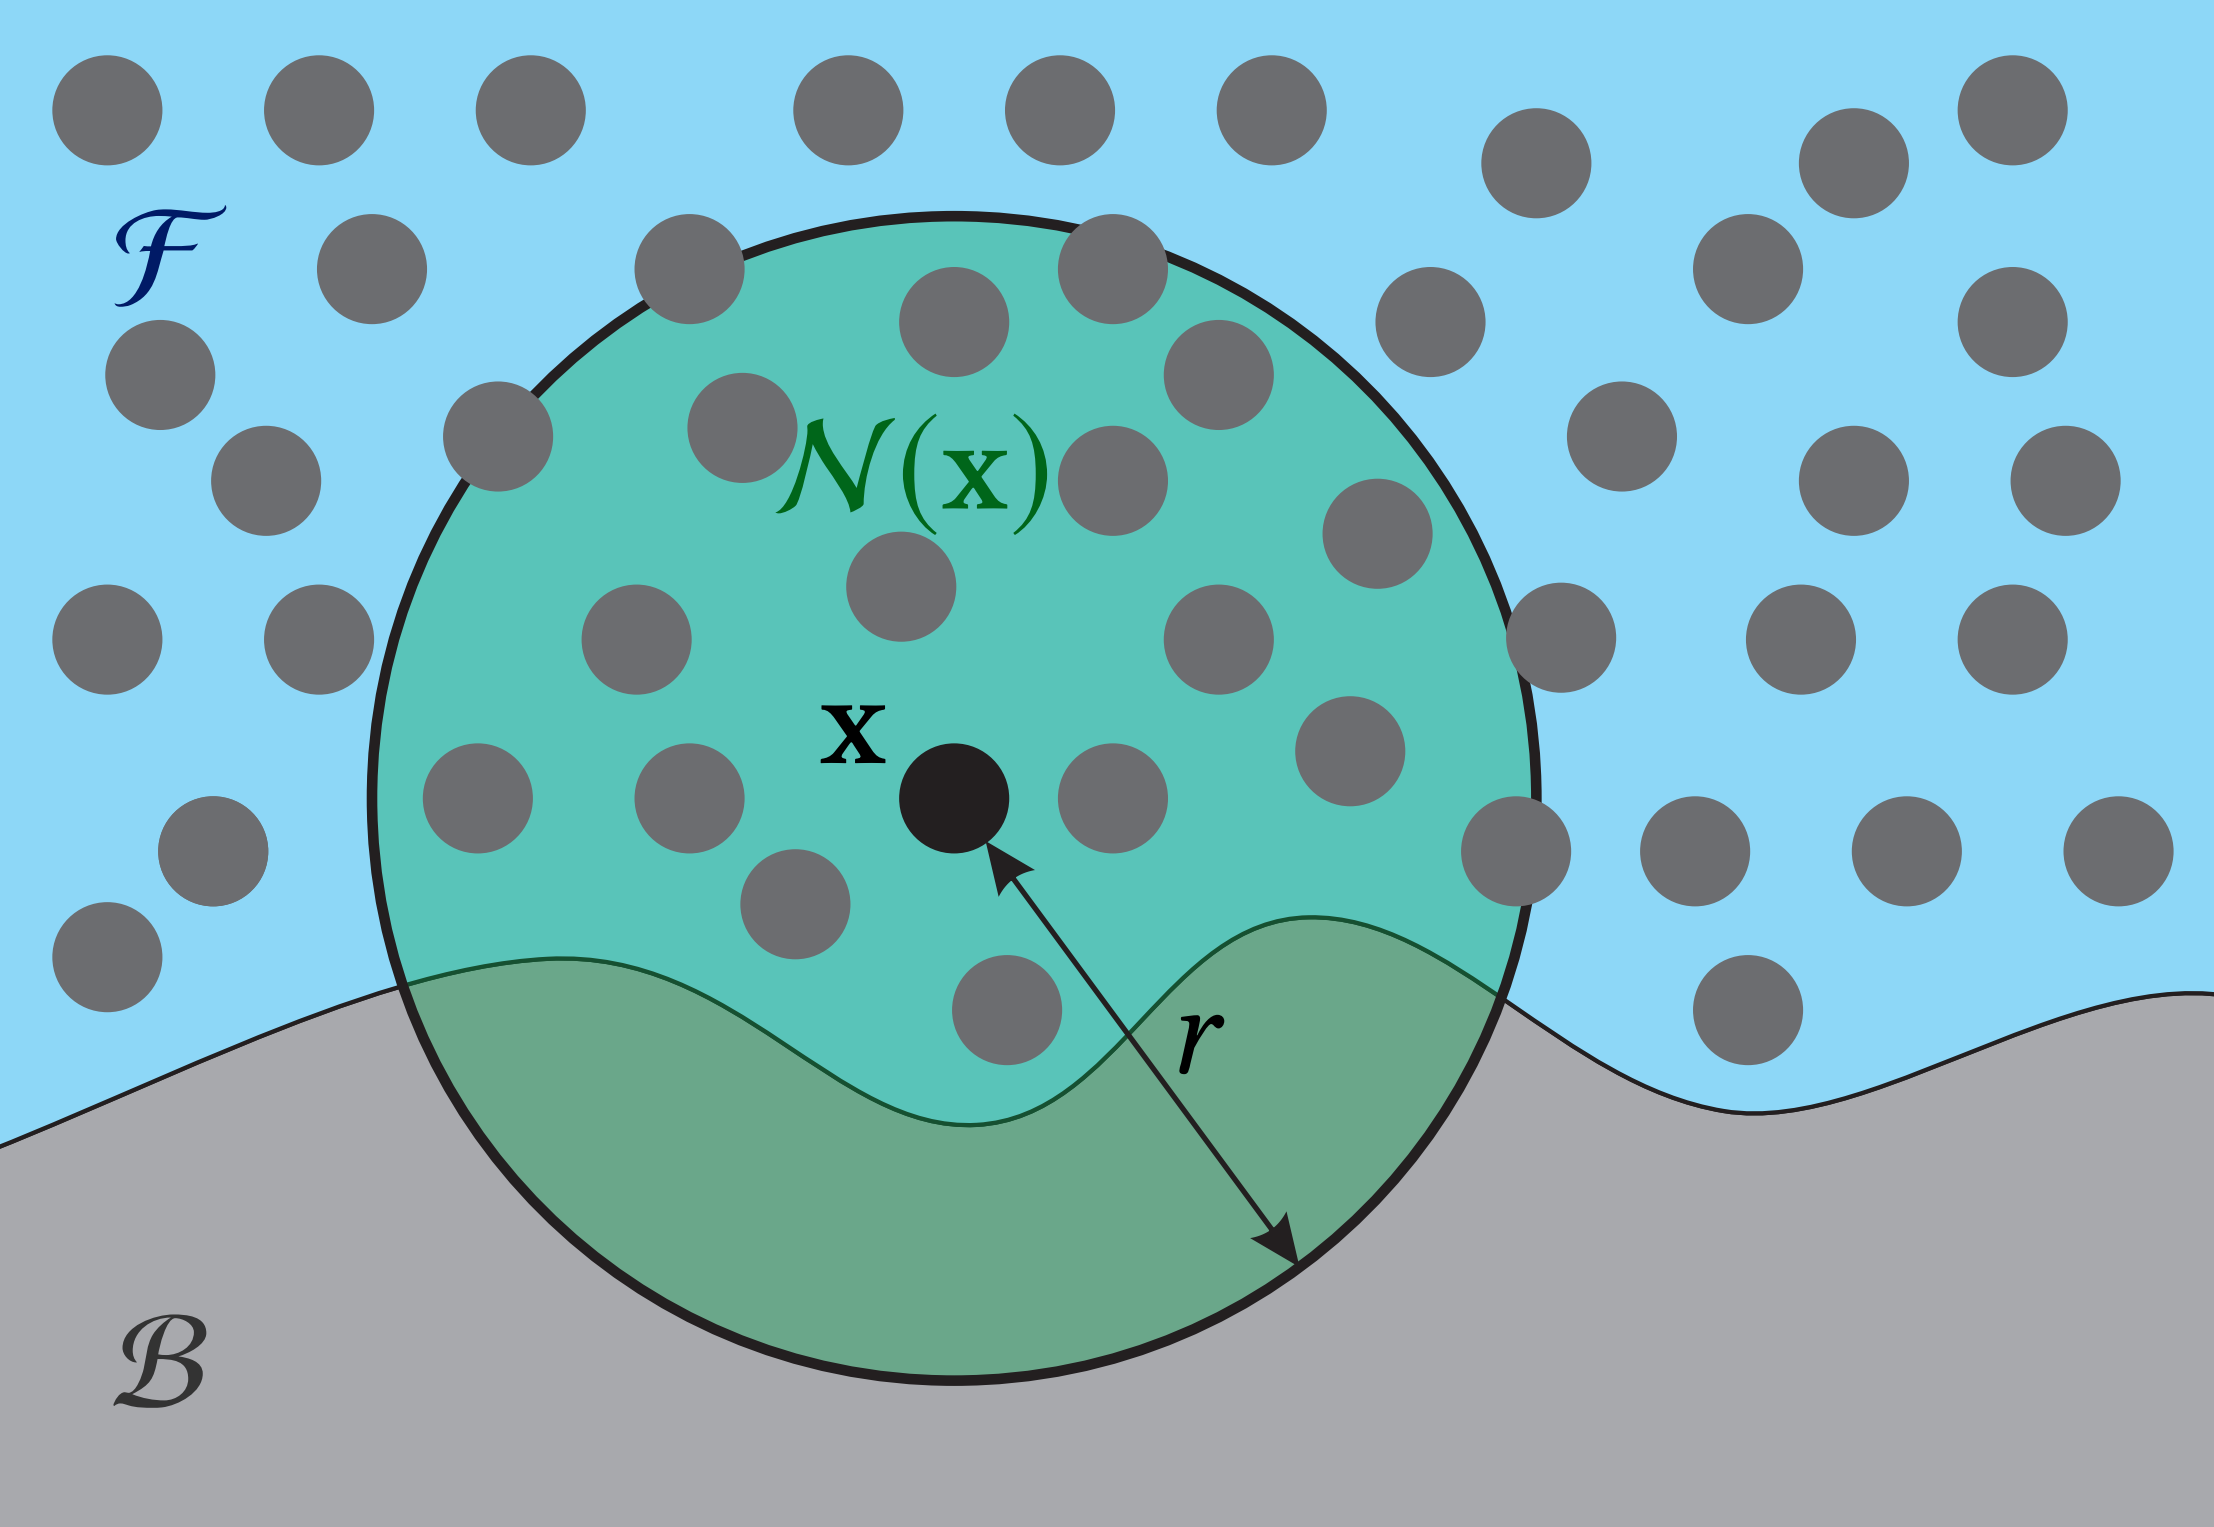
\includegraphics[width=.55\textwidth]{figures/simulation/boundary.png}
    	\caption{边界条件($\mathcal F$ 为流体,$\mathcal B$ 为固体边界,$\mathcal N(\mathbf x)$ 为粒子 $\mathbf x$ 的邻域)}
    \end{figure}

\subsubsection{密度贴图}

    公式\ref{eq:densfunc}描述了流体密度的计算公式,其在流体内部是正确的,但是在边界处由于未考虑边界固体的密度贡献从而造成欠采样,如果加上这部分贡献,密度计算公式可以表示为
    \begin{equation}\label{eq:densfuncb}
    	\begin{aligned}
    	\rho(\mathbf x) &=
    	\int_{\mathcal N (x) \cap \mathcal F} \rho(\mathbf x') W(\mathbf{x} - \mathbf{x}')\, \mathrm d \mathbf x'
    	+
    	\int_{\mathcal N (x) \cap \mathcal B} \rho(\mathbf x') W(\mathbf{x} - \mathbf{x}')\, \mathrm d \mathbf x'
    	\\
    	&= \rho_{\mathcal F}(\mathbf x) + \rho_{\mathcal B}(\mathbf x)
    	\end{aligned}
    \end{equation}
    而在具体计算边界密度贡献 $\rho_{\mathcal B}$ 时,将固体密度等同于流体初始密度 $\rho_0$,
    \begin{equation}
    	\begin{gathered}
    	\rho_{\mathcal B}(\mathbf x) =
    	\int_{\mathcal N(\mathbf x)} \phi (D(\mathbf x')) W(\mathbf{x} - \mathbf{x}') \, \mathrm d \mathbf x'
    	\\
    	\phi(d) = 
    	\left\{
    	\begin{array}{ll}
    	\rho_0 (1 - \frac {d}{h}) & \mathrm{if} \; d < h \\
    	0 & \mathrm{otherwise}
    	\end{array}
    	\right.
    	\end{gathered}
    \end{equation}
    其中 $D(\mathbf x)$ 为有向距离函数,表示 $\mathbf x$ 到边界的最短距离,如果为负值则表示 $\mathbf x$ 在固体内部,为正值则表示在固体外部流体内部。而 $\phi(d)$ 是一个简单的线性平滑函数,他将固体边界的密度影响向外扩大了 $h$,防止密度值在边界上突变。

\subsubsection{体积贴图}

    通过公式\ref{eq:densfuncb}可以很直观的计算空间各处边界固体对流体粒子的密度贡献,但是SPH模型往往要通过密度的梯度计算压强,而通过公式\ref{eq:densfuncb}计算密度梯度就相当于对核函数梯度进行积分,这会导致梯度方向计算产生误差,所以Bender等人\cite{BKW19SPHB}提出了体积贴图方法,不再计算边界密度贡献,而是计算边界体积
    \begin{equation}
    	\begin{gathered}
    	V_{\mathcal B} (\mathbf x) = 
    	\int_{\mathcal N(\mathbf x)} \phi^* (D(\mathbf x')) \, \mathrm d \mathbf x' 
    	\\
    	\phi^*(d) = 
    	\left\{
    	\begin{array}{ll}
    	\frac{W_{cubic}(d)}{W_{cubic}(0)} & \mathrm{if} \; 0 < d < h \\
    	1 & \mathrm{if} \; d \le 0 \\
    	0 & \mathrm{otherwise} \\
    	\end{array}
    	\right.
    	\end{gathered}
    \end{equation}
    体积贴图使用的平滑函数 $\phi^*$ 的定义与密度贴图的计算略有不同,式中 $W_{cubic}$ 表示三阶样条核函数\cite{MCG03SPH}。在具体实现上,我们使用高斯-勒让德积分(Gauss-Legendre quadrature)数值求解公式积分值。而针对有向距离函数 $D$ ,我们则使用了Bærentzen等人\cite{BH05SDF}提出的有向距离场(Signed Distance Field, SDF)计算方法,对SDF插值即可得到空间中任意位置的有向距离,针对SDF的空间离散与插值方法与体积贴图相同,将在3.3.3节具体介绍。我们在确定了边界体积的大小之后,可以很容易地确定边界密度的对流体粒子 $\mathbf x$ 的贡献
    \begin{equation}
    	\rho_{\mathcal B}(\mathbf x) =
    	V_{\mathcal B} (\mathbf x) \rho_0 W(\mathbf x - \mathbf x^*)
    \end{equation}
    上式中 $\mathbf x^*$ 是距离 $\mathbf x$ 最近的边界点,可以由SDF反推得知。
    
    结合上一节中阐述的PBF流体仿真算法,可以将边界密度贡献添加到PBF的密度约束中(公式\ref{eq:constrainsys}),这样 $\lambda_i$ 的计算公式(公式\ref{eq:lambda2})就变为了
    \begin{equation}
    	\lambda_i = - \frac 
    	{ \max(\rho_i^{\mathcal F} / \rho_0 + V_i^{\mathcal B} W(\mathbf x_i - \mathbf x_i^*) - 1, 0) }
    	{ \frac {1}{\rho_0^2} (|\sum_j m_j \nabla W_{ij}|^2 + \sum_j |m_j \nabla W_{ij}|^2 ) + \varepsilon }
    \end{equation}
    同样可以得到边界条件对PBF中位置更新向量的影响为
    \begin{equation}
    	\Delta \mathbf x_{\mathcal B} = \frac{1}{2} \lambda_i V_{\mathcal B}(\mathbf x) \nabla W(\mathbf x - \mathbf x^*)
    \end{equation}
    则加入边界条件影响的位置更新向量计算公式会变为
    \begin{equation}
    	\Delta \mathbf x_i \approx
    	\frac{1}{2\rho_0} \sum_j (m_i \lambda_i + m_j \lambda_j) \nabla W_{ij} +
    	\frac{1}{2} \lambda_i V_i^{\mathcal B} \nabla W(\mathbf x_i - \mathbf x_i^*)
    \end{equation}
    
    \begin{figure}
    	\centering
    	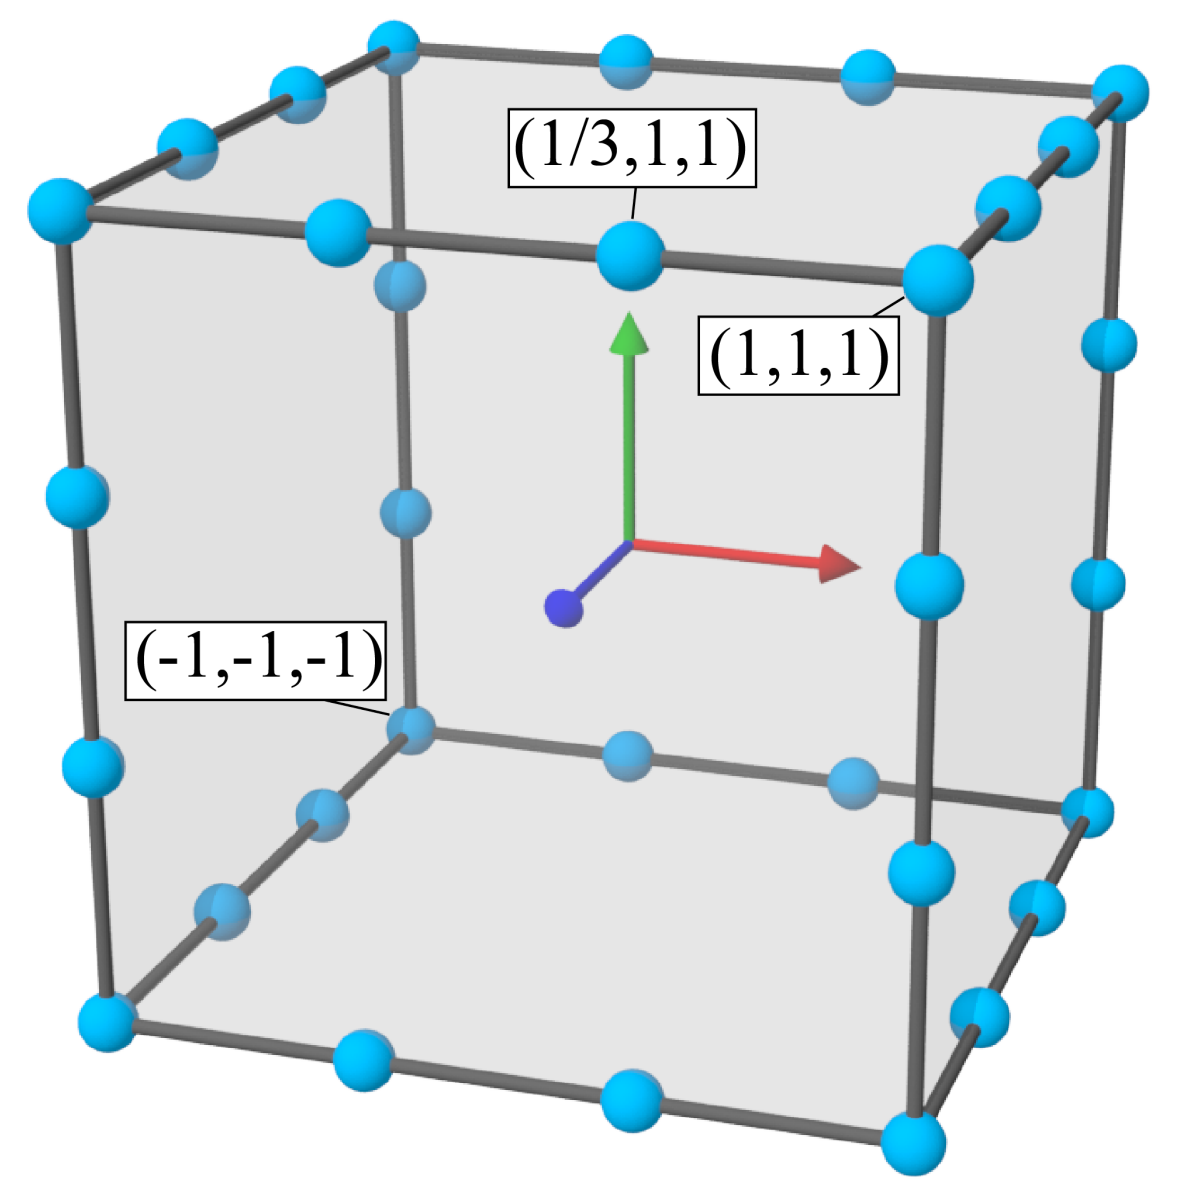
\includegraphics[width=.4\textwidth]{figures/simulation/sample.png}
    	\caption{三次多项式插值}
    	\label{fig:cubicsample}
    \end{figure}

\subsubsection{空间离散}
    在具体实现上,本文使用六面体网格划分空间,并采用Bender等人\cite{BKW19SPHB}推荐的Serendipity类型三次多项式离散化边界体积。查询空间中任意位置的边界体积值需要插值32个采样点(如图\ref{fig:cubicsample})。插值函数定义如下:
    \begin{equation}\label{eq:samplefunc}
    	f(\mathbf x') \approx \sum_{i=1}^{32} w_i(\mathbf x') s_i \qquad \mathbf x' \in [-1,1]^3 
    \end{equation}
    在插值计算时需要注意,要先将粒子位置转换到以六面体网格为中心的局部坐标中,具体计算方式为 $\mathbf x' = [\mathrm{diag}(\mathbf b - \mathbf a)]^{-1}(2\mathbf x -(\mathbf a + \mathbf b))$,$\mathbf a,\; \mathbf b$分别为此六面体最大和最小格点位置。公式\ref{eq:samplefunc}中 $s_i$ 为采样点数据,$w_i$ 为型函数(Shape Function),其计算结果为插值权重,定义如下
    \begin{equation}
    	w_i(\mathbf x) =
    	\left\{
    	\begin{array}{lll}
    
    	\frac{1}{64} (1 + \xi x)(1 + \eta y)(1 + \zeta z) \left[ 9(x^2 + y^2 + z^2)-19 \right] 
    	& \mathrm{corner} & (\xi,\eta,\zeta=\pm 1) \\
    
    	\frac{9}{64} (1 - x^2) (1 + 9 \xi x) (1 + \eta y) (1 + \zeta z)
    	& x\; \mathrm{edge} & (\xi=\pm \frac{1}{3} \quad \eta,\zeta=\pm 1) \\
    
    	\frac{9}{64} (1 - y^2) (1 + \xi x) (1 + 9 \eta y) (1 + \zeta z)
    	& y\; \mathrm{edge} & (\eta=\pm \frac{1}{3} \quad \xi,\zeta=\pm 1)\\
    
    	\frac{9}{64} (1 - z^2) (1 + \xi x) (1 + \eta y) (1 + 9 \zeta z)
    	& z\; \mathrm{edge} & (\zeta=\pm \frac{1}{3} \quad \xi,\eta=\pm 1) \\
    
    	\end{array}
    	\right.
    \end{equation}
    其中 $(\xi,\,\eta,\,\zeta)$ 为采样点坐标。
    
    \begin{figure}
    	\centering
    	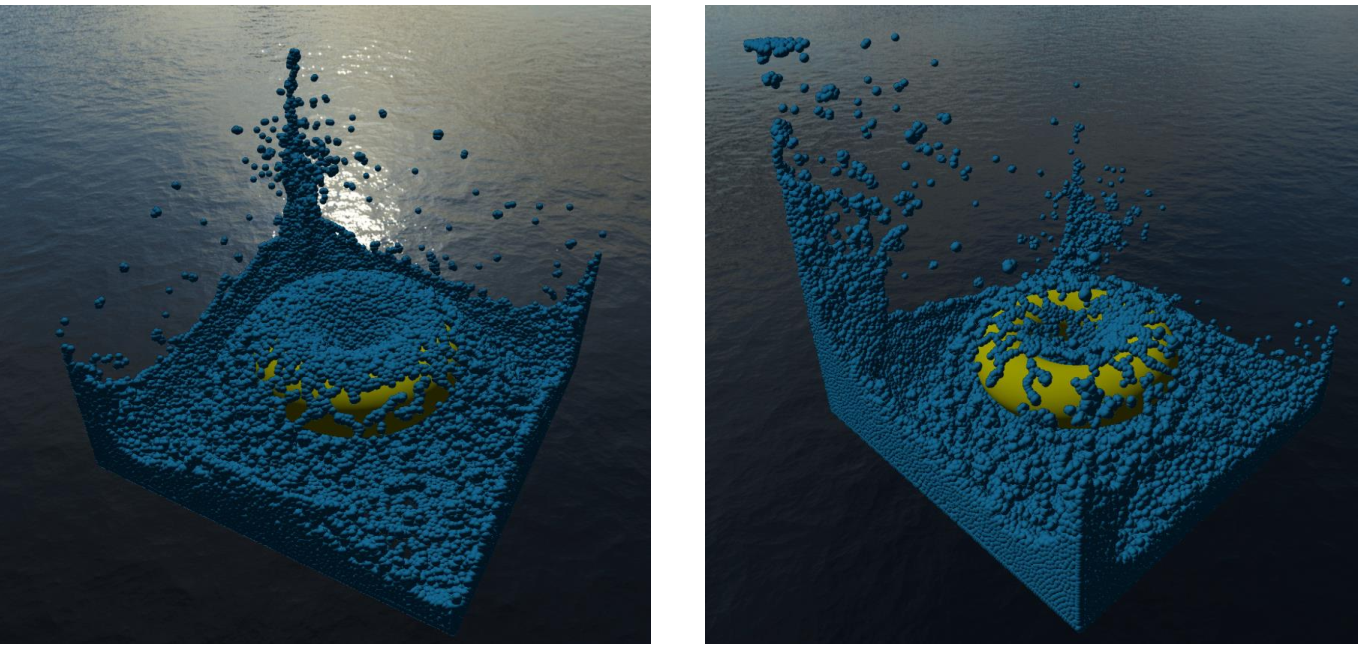
\includegraphics[width=.95\textwidth]{figures/simulation/boundary_sample.pdf}
    	\caption{固体圆环边界与流体粒子交互}
    \end{figure}

\subsection{本章小结}
    本章主要阐述了不可压缩流体的模拟算法。首先介绍了SPH方法,如何从粒子视角离散近似物理场及其梯度场。接下来以基于位置的动力学的思想为基础,推导了PBF在密度恒定约束下的粒子位置迭代公式。最后介绍了一种隐式边界条件表示方法——体积贴图法,并将其添加到PBF的框架中。总的来说,本章的核心是PBF,一种直接改变粒子位置的迭代式压强求解方法,它稳定且高效,适用于实时不可压缩流体仿真。
\clearpage
\section{流体非压强力模型}
    第三章中通过位置约束的求解即可得到一个高效稳定的不可压缩流体的仿真框架。不过由于离散采样、近似误差等原因使得模拟效果真实感不强,产生了诸如粒子内聚力太低、粒子抖动、涡量不守恒等问题。本章将通过严谨的物理建模或启发式的经验公式来解决这些问题,比如表面张力、人工粘性、涡量补偿等。这些方法均在压强求解后计算,统称为非压强受力。这部分我们不再采用位置约束求解而是基于传统的物理定律,计算每种力产生的加速度,再通过时间积分改变粒子的速度与位置。
    
    \begin{figure}[htbp]
    	\centering
    	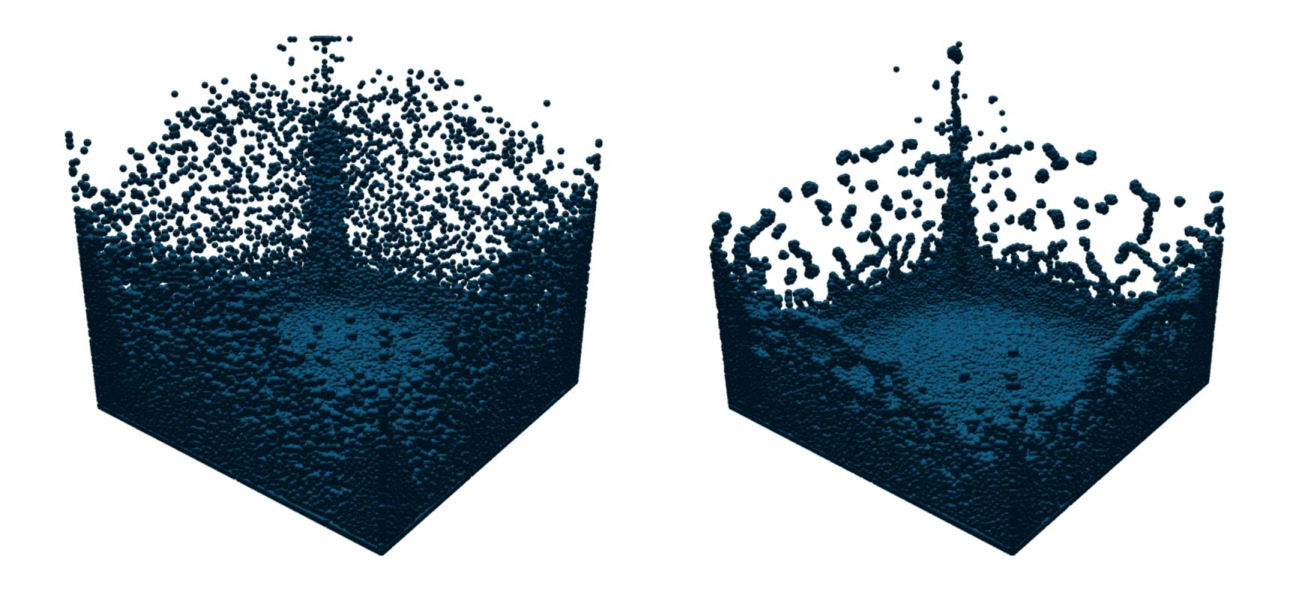
\includegraphics[width=.99\textwidth]{figures/simulation/tension.pdf}
    	\caption{关闭表面张力(左)开启表面张力(右)}
    \end{figure}

\subsection{表面张力}
    表面张力是一种重要的物理现象,在日常生活中普遍存在。它是微观尺度上液体分子间相互吸引的结果。分子在流体内部相互吸引,而表面的分子被向内拉。因此,表面张力会使流体表面积最小化,比如,当排除外力时水滴会形成球体(如图\ref{fig:tensionsphere})。Akinci等人\cite{AAT13SPH}在微观尺度计算粒子内聚力,宏观尺度最小化流体表面积,同时考虑这两种因素来建模流体表面张力。

\subsubsection{内聚力}
    粒子内聚力可以由粒子与其近邻粒子之间的位置差来确定,其计算公式为
    \begin{equation}
    	\mathbf F_{i \leftarrow j} ^{cohesion}
    	= - m_i m_j
    	\frac {\mathbf x_i - \mathbf x_j} {\mathbf x_i - \mathbf x_j}
    	W_{cohesion} (|\mathbf x_i - \mathbf x_j|)
    \end{equation}
    其中 $W_{cohesion}$ 是为计算内聚力而设计的特殊核函数,在采样点据核函数中心过近时会取得负值,在 $|\mathbf r| = 0.5h$ 时取得最大值。这样在粒子间距过小时产生排斥力,防止粒子聚集,而在其间距过大时内聚力趋近于0,对距离较远的粒子也没有影响,仅当粒子间距在一定范围内时,内聚力才有较大影响。其具体定义如下
    \begin{equation}
    	W_{cohesion}(\mathbf r, h) = \frac {32} {\pi h^9}
    	\left\{
    	\begin{array}{ll}
    
    	(h - |\mathbf r|)^3 |\mathbf r|^3 & 0.5h < |\mathbf r| \le h \\
    	2(h - |\mathbf r|)^3 |\mathbf r|^3 - \frac {h^6} {64} & 0 < |\mathbf r| \le 0.5h \\
    	0 & \mathrm{otherwise} \\
    
    	\end{array}
    	\right.
    \end{equation}
    
    \begin{figure}
    	\centering
    	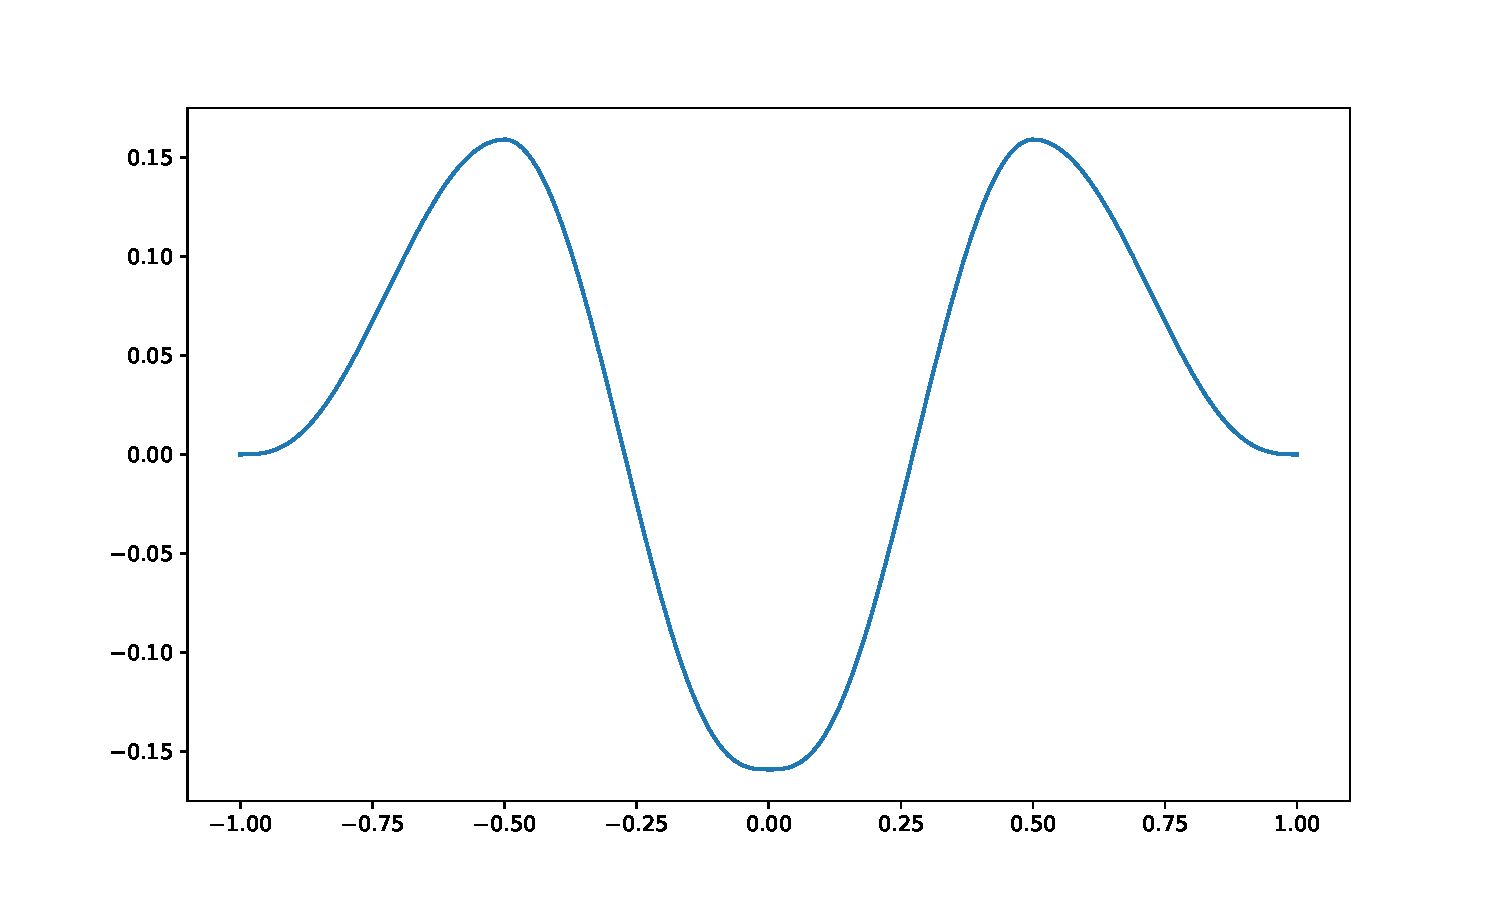
\includegraphics[width=.85\textwidth]{figures/simulation/cohesion_kernel.pdf}
    	\caption{内聚力核函数示意图}
    \end{figure}
    
    \begin{figure}[bp]
    	\centering
    	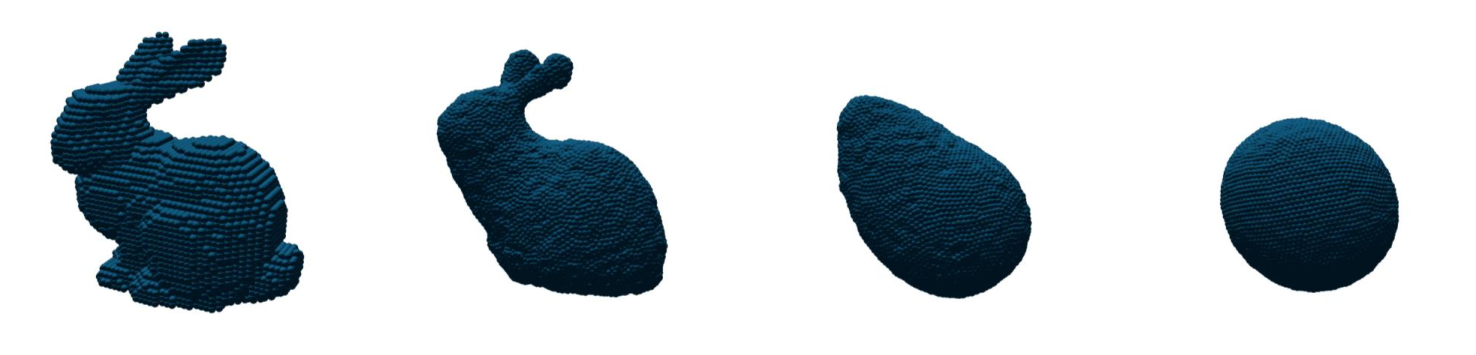
\includegraphics[width=.99\textwidth]{figures/simulation/surface.pdf}
    	\caption{流体粒子在没有重力的环境中形成球形}
    	\label{fig:tensionsphere}
    \end{figure}

\subsubsection{最小化表面积}
    在微观尺度上计算粒子内聚力仍不足以最小化流体表面积,因此Akinci等人设计了额外的力来抵消表面的曲率变化,定义如下
    \begin{equation}\label{eq:curvature}
    	\mathbf F_{i \leftarrow j} ^{curvature} =
    	- m_i (\mathbf n_i - \mathbf n_j)
    \end{equation}
    其中 $\mathbf n$ 为粒子法向。对于法向的计算,可以采样平滑颜色场的思路,具体来说,将粒子颜色设为1,而其他区域均记为0,那么计算这个平滑颜色场的梯度就可以得到此粒子的法向
    \begin{equation}
    	\mathbf n_i = h \sum_j \frac {m_j} {\rho_j} \nabla W_{ij}
    \end{equation}
    如果粒子在流体内部,显然上式计算结果趋近于0,而粒子在流体表面时,计算结果为指向表面外的向量,方向与表面曲率大小成正比。将其代入公式\ref{eq:curvature}可以发现,粒子受力在流体内部与较平整的流体表面计算结果均为0,曲率越大时,受力也越大。
    
    最终结合微观与宏观尺度的受力模型,表面张力计算公式为
    \begin{equation}
    	\mathbf F_{i} ^{surface\;tension} =
    	\alpha \sum_j K_{ij} (\mathbf F_{i \leftarrow j} ^{cohesion} + \mathbf F_{i \leftarrow j} ^{curvature})
    \end{equation}
    其中 $\alpha$ 为用户指定的表面张力参数,$K_{ij} = \frac {2\rho_0} {\rho_i + \rho_j}$ 是一个对称的缩放因子,在密度计算值偏低的流体表面放大表面张力的影响。

\subsection{涡量补偿}
    湍流是流体运动中最具视觉吸引力的现象之一,它是由于不同尺度上流体速度场的涡量产生的。在密度约束解算中,会引入许多额外的阻尼,产生能量耗散,所以流体速度场涡量也往往难以保持。Macklin等人\cite{MM13PBF}采用涡量补偿(Vorticity Confinement)的方法对流体系统注入额外能量
    \begin{equation}
    	\mathbf F_i ^{vorticity} =
    	\gamma (\frac{\eta_i}{|\eta_i|} \times \omega_i) \\
    	\eta_i = \nabla |\omega_i| = \sum_j \frac {m_j} {\rho_j} |\omega_j| \nabla W_{ij}
    \end{equation}
    其中 $\omega$ 为涡量,其计算公式如下
    \begin{equation}
    	\omega_i = \nabla \times \mathbf v =
    	\sum_j \mathbf v_{ij} \times \nabla W_{ij}
    \end{equation}
    
    \begin{figure}[htbp]
    	\centering
    	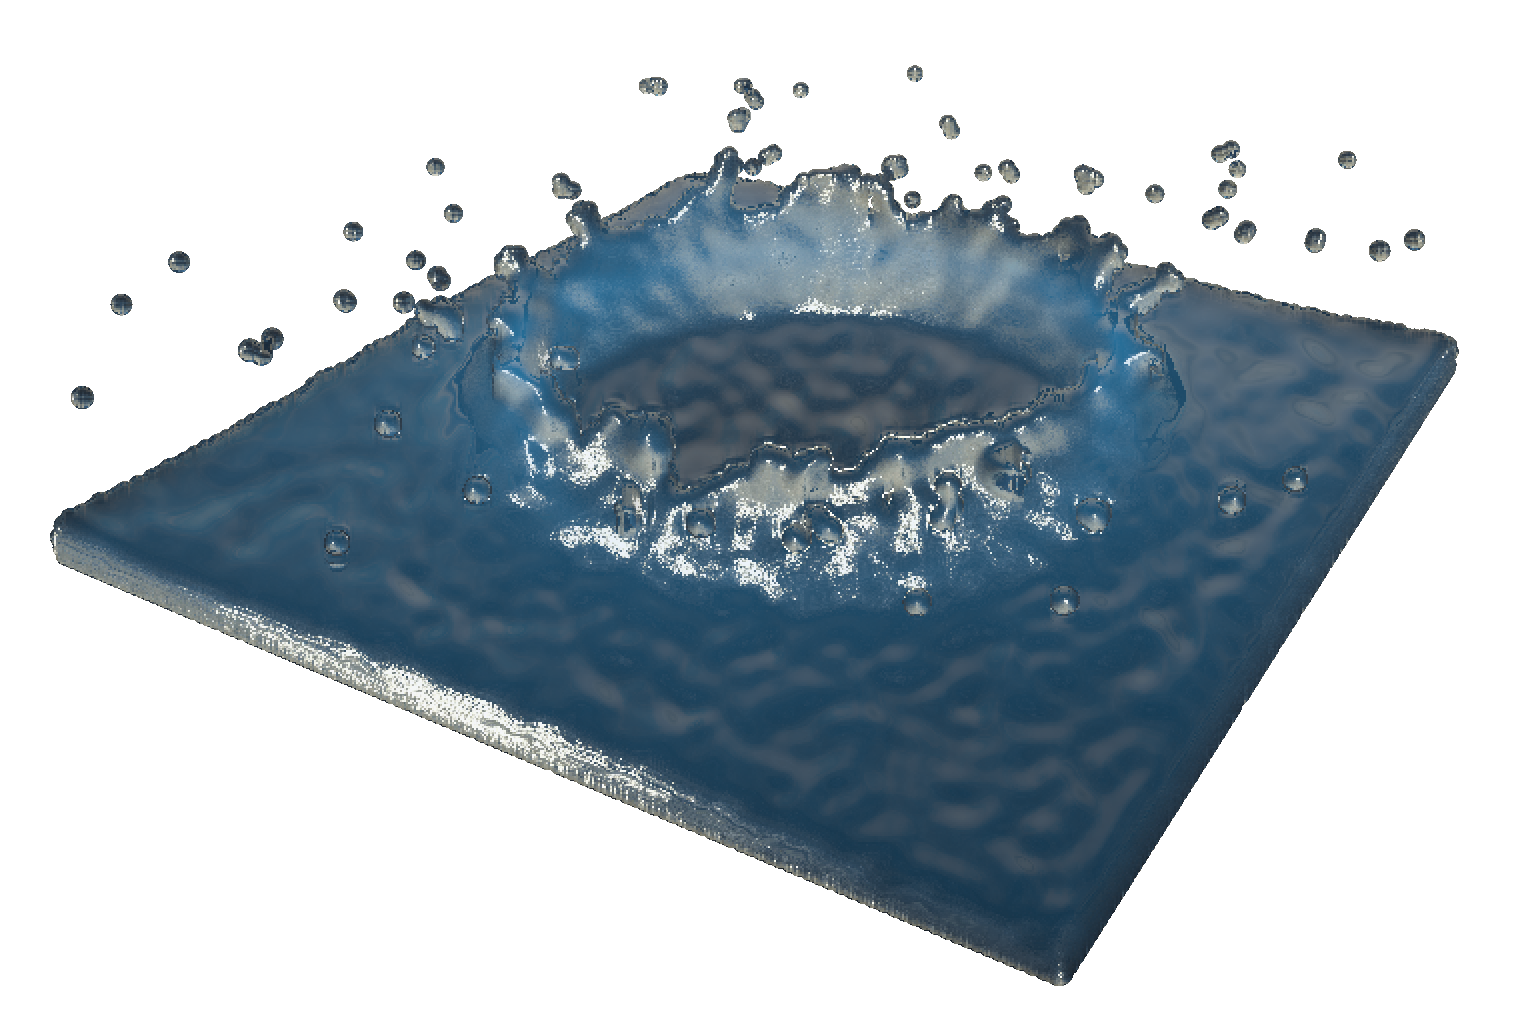
\includegraphics[width=.7\textwidth]{figures/simulation/drop.png}
    	\caption{在非压强力作用下的水滴掉落场景}
    \end{figure}

\subsection{人工粘性}
    PBF的位置约束推导是以密度不变为核心的,理论上这相当于速度场散度为0,即满足流体不可压缩条件。但在实际计算过程中,由于没有对流体速度场做相应约束,会导致速度场中存在高频噪声,反应到模拟效果上就是流体粒子在不停地小幅震动。Bender等人提出的DFSPH\cite{BK15DFSPH}方法通过同时求解密度和速度散度这两个约束条件完全解决了这个问题。但出于性能考虑,本文通过引入人工粘性XSPH\cite{SB2012XSPH}来缓解这种现象,简单来说,XSPH相当于对流体速度场做了一次模糊操作,减少了高频噪声,其计算过程如下
    \begin{equation}
    	\mathbf v_i' = \mathbf v_i + \beta \sum_j \mathbf v_{ij} \cdot W_{ij}
    \end{equation}
    其中 $\beta$ 为指定的粘性系数,$\mathbf v_{ij}$ 为粒子间速度之差,即 $\mathbf v_{ij} = (\mathbf v_i - \mathbf v_j)$ 。这种显示更新速度的方式在时间步较大时并不稳定,所以人工粘性只适用于水这种几乎没有粘性的流体,而蜂蜜等高粘性流体需要隐式积分的处理方式。

\subsection{本章小结}
    本章主要阐述了SPH框架中三种非压强力,分别是表面张力、涡量补偿力与粘性力。其中本章从宏观和微观两种角度下分别推导了对应的约束力公式,组合在一起形成表面张力公式。而涡量补偿本质上是向系统中注入新的能量用于抵消数值计算产生的阻尼,保证了流体速度场涡量守恒。最后,粘性力用于去除流体速度场的高频噪声,防止粒子抖动。这些非压强受力均在流体压强解算后施加,用于增强流体仿真的真实感和稳定性。
\clearpage
\section{高效邻域粒子查找算法}
    SPH方法以粒子作为采样点来离散采样空间中的物理量,如速度、密度、压强、作用力等等。这些物理量又需要其他粒子通过核函数加权求和来确定。而核函数是紧支撑的,所以在计算是仅需要确定每个粒子周围的邻域粒子集合即可,这是SPH流体模拟中非常重要的一个步骤,它的准确性和效率直接影响到SPH的仿真稳定性,计算精度和速度。
    
    \begin{figure}[htbp]
    	\centering
    	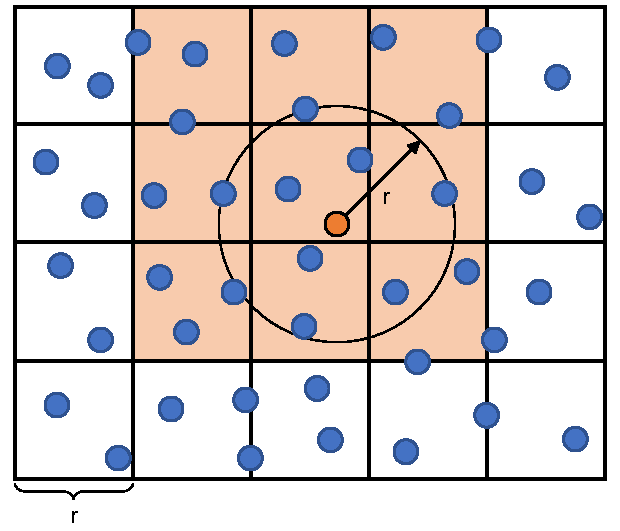
\includegraphics[width=.35\textwidth]{figures/neighbor/uniform_grid.pdf}
    	\caption{均匀网格划分}
    \end{figure}

\subsection{方法概述}
    查找邻域粒子的过程可以分为两个阶段,第一阶段是对每个粒子构建邻域粒子索引集合,第二阶段是在计算物理量时直接通过这个集合查找邻域粒子。查找阶段的时间复杂度是 $O(mn)$,$m$ 为邻域粒子的最大数量,在具体实现时是一个确定的常数,所以查找阶段可以达到线性复杂度 $O(n)$。而对于索引集合的构建,穷举算法的时间复杂度是 $O(n^2)$,SPH模拟中仿真粒子的数量非常大,这样做的性能开销是往往不可接受的,所以这个阶段是算法优化的重点。
    
    优化算法的基本思路是,将空间划分为均匀网格,找到每个网格中包含的所有粒子,然后在确定邻域粒子集合时,只需要计算周围网格中包含的粒子即可。如果网格中粒子最大数量为 $k$,则优化算法的时间复杂度为 $O(kn)$。
    
    具体来说,如果核函数半径为 $r$(即邻域搜索半径为 $r$),可以将空间划分为间距为 $r$ 的网格。在计算粒子 $p$ 的邻域粒子集合时,仅需要查找 $p$ 所在网格与相邻网格中的粒子,在三维空间中共27个网格。算法实现共分为两个步骤,空间网格划分和构建邻域粒子集合。这两个步骤所涉及的数据结构在逻辑上可以抽象为一种,将下一节详细介绍。

    \begin{figure}
    	\centering
    	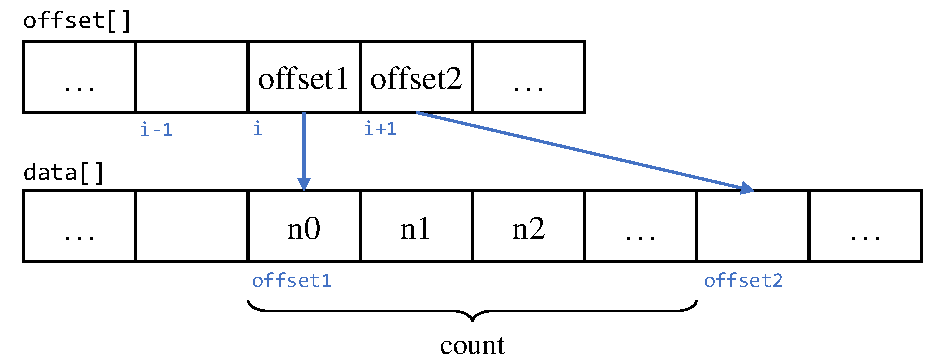
\includegraphics[width=.55\textwidth]{figures/neighbor/data_structure.pdf}
    	\caption{集合数组数据结构}
    \end{figure}

    \begin{table}
	\centering
	\caption{集合数组存储格式对比}
	\begin{tabular}{lll}
	\toprule
	数据结构 & 优点 & 缺点 \\
	\midrule
	\multirow{2}{*}{定长格式}
	& 1. 实现简单。  & 1. 存储空间消耗大。  \\
	& 2. 支持随机存取。  & 2. 存储碎片化,读取效率较低。  \\
	\hline
	\multirow{3}{*}{不定长格式} 
	& 1. 支持随机存取。  & 1. 实现较复杂。 \\
	& 2. 存储空间无额外消耗。  & 2. 写入时需要额外的计算步骤。  \\
	& 3. 存储连续,读取效率高。  &   \\
	\bottomrule
	\end{tabular}
\end{table}

\subsection{集合数组}
\subsubsection{数据结构}
    邻域粒子集合和空间网格划分集合的存储数据具有一定相似结构,它们都需要存储确定数量个集合,但每个集合的元素数量不定,我们将这种抽象结构定义为集合数组。具体来说,对于邻域粒子集,粒子数量是确定的,但每个粒子邻域中的粒子数量不定。对于空间网格划分集,均匀划分后网格数量是确定的,但每个网格中粒子数量不定。如果是CPU实现,可以考虑邻接表等高级数据结构,但是对于GPU程序,需要考虑存储空间排布、并行随机读写效率等问题。这种数据结构的实现有两种格式,定长格式和不定长格式。
    
    定长格式确定了集合元素的数量上限,对于每个集合所消耗的存储空间相同。其优点为实现简单,支持随机读写。缺点为存储空间消耗较大,需要预设一个集合数量;并且存储碎片化严重,空间局部性差,难以充分利用硬件性能。
    
    不定长格式与此相反,长度不定的集合之间连续存储,可以降低存储消耗,无存储碎片。但缺点为实现较复杂,需要offset[]额外数组辅助来支持并行随机读取,在并行构建时也需要先行确定这两个数组中的数据,再写入数据。
    
    不定长格式的数据结构在存储开销的优势使得其更适合浏览器环境的流体模拟。虽然其构建开销较高,但是实际实现中数据读取次数远大于构建次数,这使得其读取效率方面的优势更为重要。

    \begin{figure}[htbp]
    	\centering
    	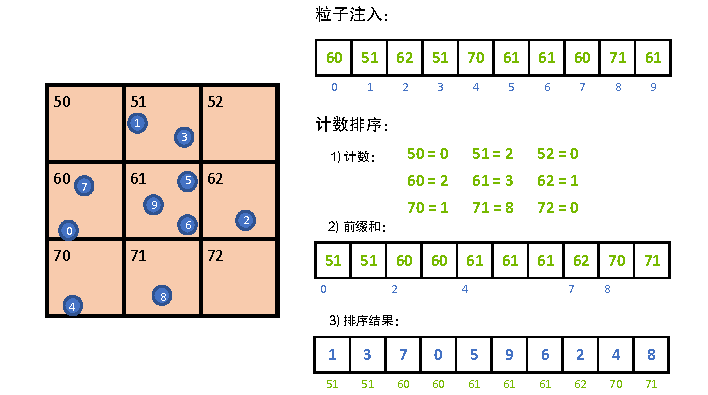
\includegraphics[width=.8\textwidth]{figures/neighbor/counting_sort.pdf}
    	\caption{计数排序}
    \end{figure}

\subsubsection{构建算法}
    最终算法实现的重要步骤就在于这两个集合数组的构建。构建邻域粒子集较简单,可以以集合为单位分配线程,在每个线程中串行地依次确定集合元素。而构建空间网格划分集较复杂,需要以集合元素为单位分配线程,在每个线程中只能确定该元素属于哪个集合,线程间还存在依赖关系。参考\cite{G10NS}和\cite{RC14NS}的方案,我们使用计数排序来确定最终结果。
    
    最终邻域粒子查找算法的计算管线为:

    \begin{enumerate}
    	\item 粒子注入,计算粒子所属网格以及网格粒子数。
    	\item 计算网格粒子数的前缀和。
    	\item 计数排序,得到空间网格划分集和。
    	\item 计算邻域粒子数量。
    	\item 计算邻域粒子数量的前缀和。
    	\item 得到邻域粒子集合。
    \end{enumerate}

    管线中2,5步骤需要计算数组前缀和,这部分将在下一节详细介绍。其他步骤并行度均等同于粒子数量,全部使用WebGPU计算管线实现。

    \begin{figure}
    	\centering
    	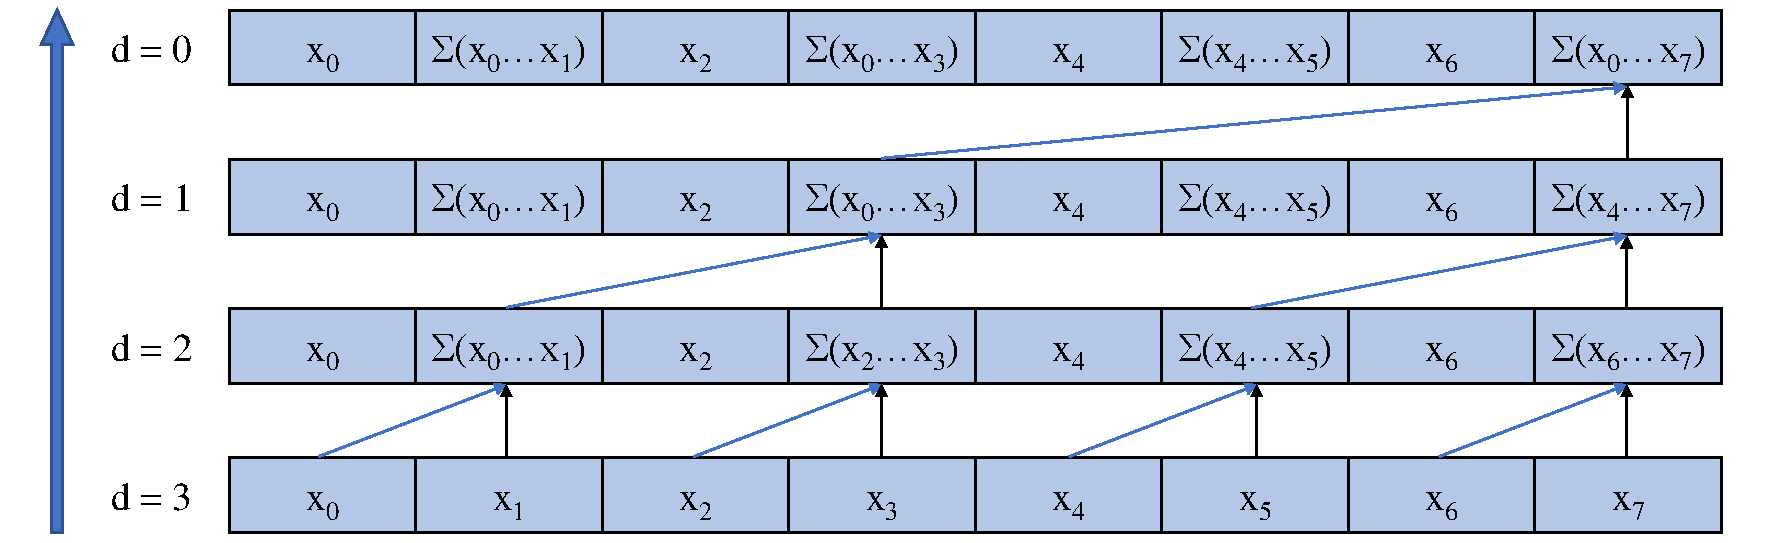
\includegraphics[width=.8\textwidth]{figures/neighbor/up_sweep.pdf}
    	\caption{自底向上扫描}
    	\label{fig:upsweep}
    \end{figure}
    
    \begin{figure}
    	\centering
    	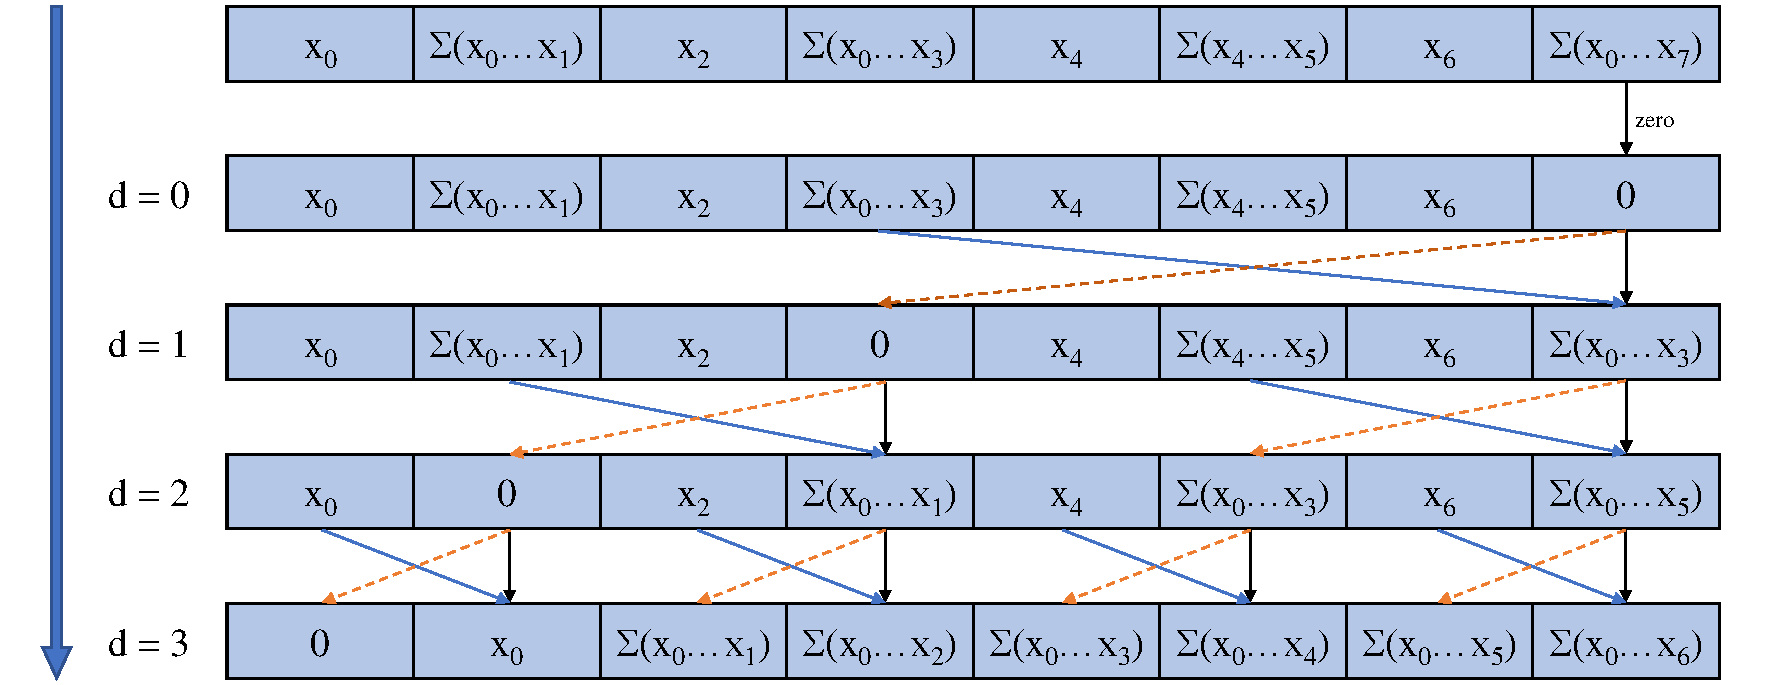
\includegraphics[width=.8\textwidth]{figures/neighbor/down_sweep.pdf}
    	\caption{自顶向下扫描}
    	\label{fig:downsweep}
    \end{figure}

\subsection{并行计算前缀和}
    对数组计算前缀和,如果是CPU串行执行,这一算法非常简单,只需要遍历一次数组即可。但是如果使用GPU并行计算大数组前缀和,就需要重新设计算法并依据硬件架构作出相应优化,才能发挥出GPU强大的并行计算能力。本文实现的前缀和算法主要参考了英伟达在CUDA上的实现\cite{HSO07SCAN} ,同时根据WebGPU的诸多限制与邻域粒子查找这一确定的应用场景,对原算法做出了相应的简化与调整。
    
    算法的基本思路为:在输入数据上建立一个平衡的二叉树(将输入数据视作二叉树叶子节点),先自底向上再自顶向下扫描两遍二叉树节点来计算前缀和。如果一个二叉树有 $n$ 个叶子节点,则树的深度为 $\log n$,每层有 $2^n$ 个节点,所以遍历一遍二叉树的计算复杂度为 $O(n)$。需要强调的是,二叉树只是算法的逻辑结构,在实际实现中并不需要构建复杂的数据结构,也不需要额外的空间存储二叉树内部节点的值。
    
    在自底向上扫描(如图\ref{fig:upsweep})阶段,每个中间节点只保存数组的部分前缀和,即此中间节点对应的叶子节点之和。
    
    在自顶向下扫描(如图\ref{fig:downsweep})阶段,每个中间节点可以根据父结点和兄弟节点的值得到完整前缀和。

    \begin{figure}
    	\centering
    	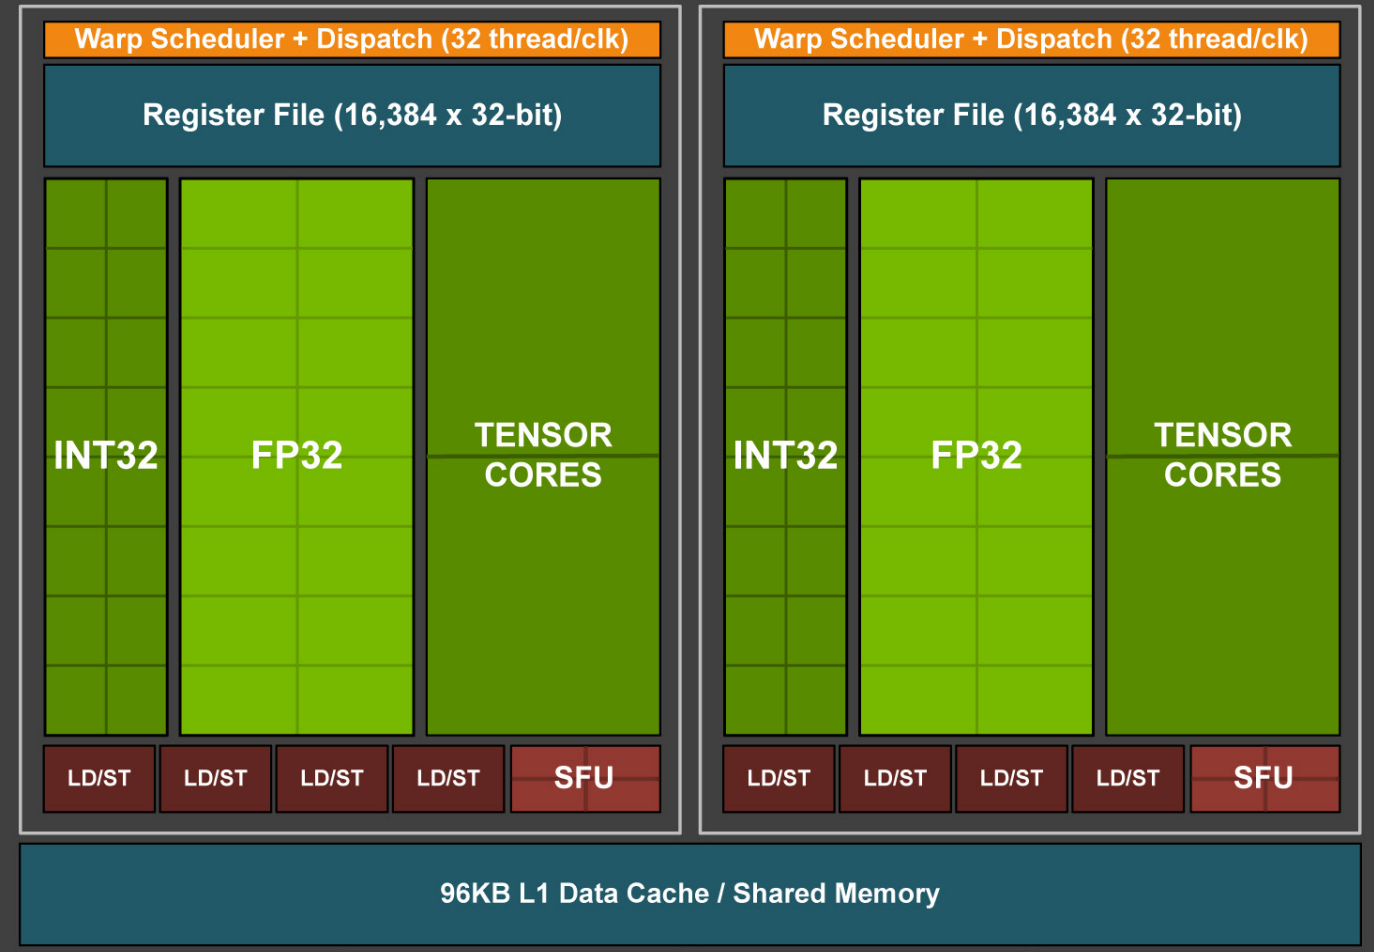
\includegraphics[width=.6\textwidth]{figures/neighbor/sm_cut.png}
    	\caption{NIVIDA Turing GPU 架构\cite{NV18Truing}}
    	\label{fig:turing}
    \end{figure}

\subsubsection{访存优化}
    GPU的存储结构(如图\ref{fig:turing})和CPU类似,同样有多级存储机制,数据主要存储在显存中,读写显存都需要花费大量时钟周期。而缓存的读写速度就会远远快于显存。GPU具有大量计算单元,称为流处理器(Stream Processor, SP),多个流处理器组成一个流多处理器(Stream Multiprocessor, SM)。一个SM有一块缓存,为SM内所有流处理器共享,称为共享内存(Shared Memory)。一般一个SM对应一个计算着色器的线程组,所以可以在一个线程组中将所有数据先载入共享内存,再完成前缀和计算,最后将共享缓冲区的计算结果写回显存。

    \begin{figure}
    	\centering
    	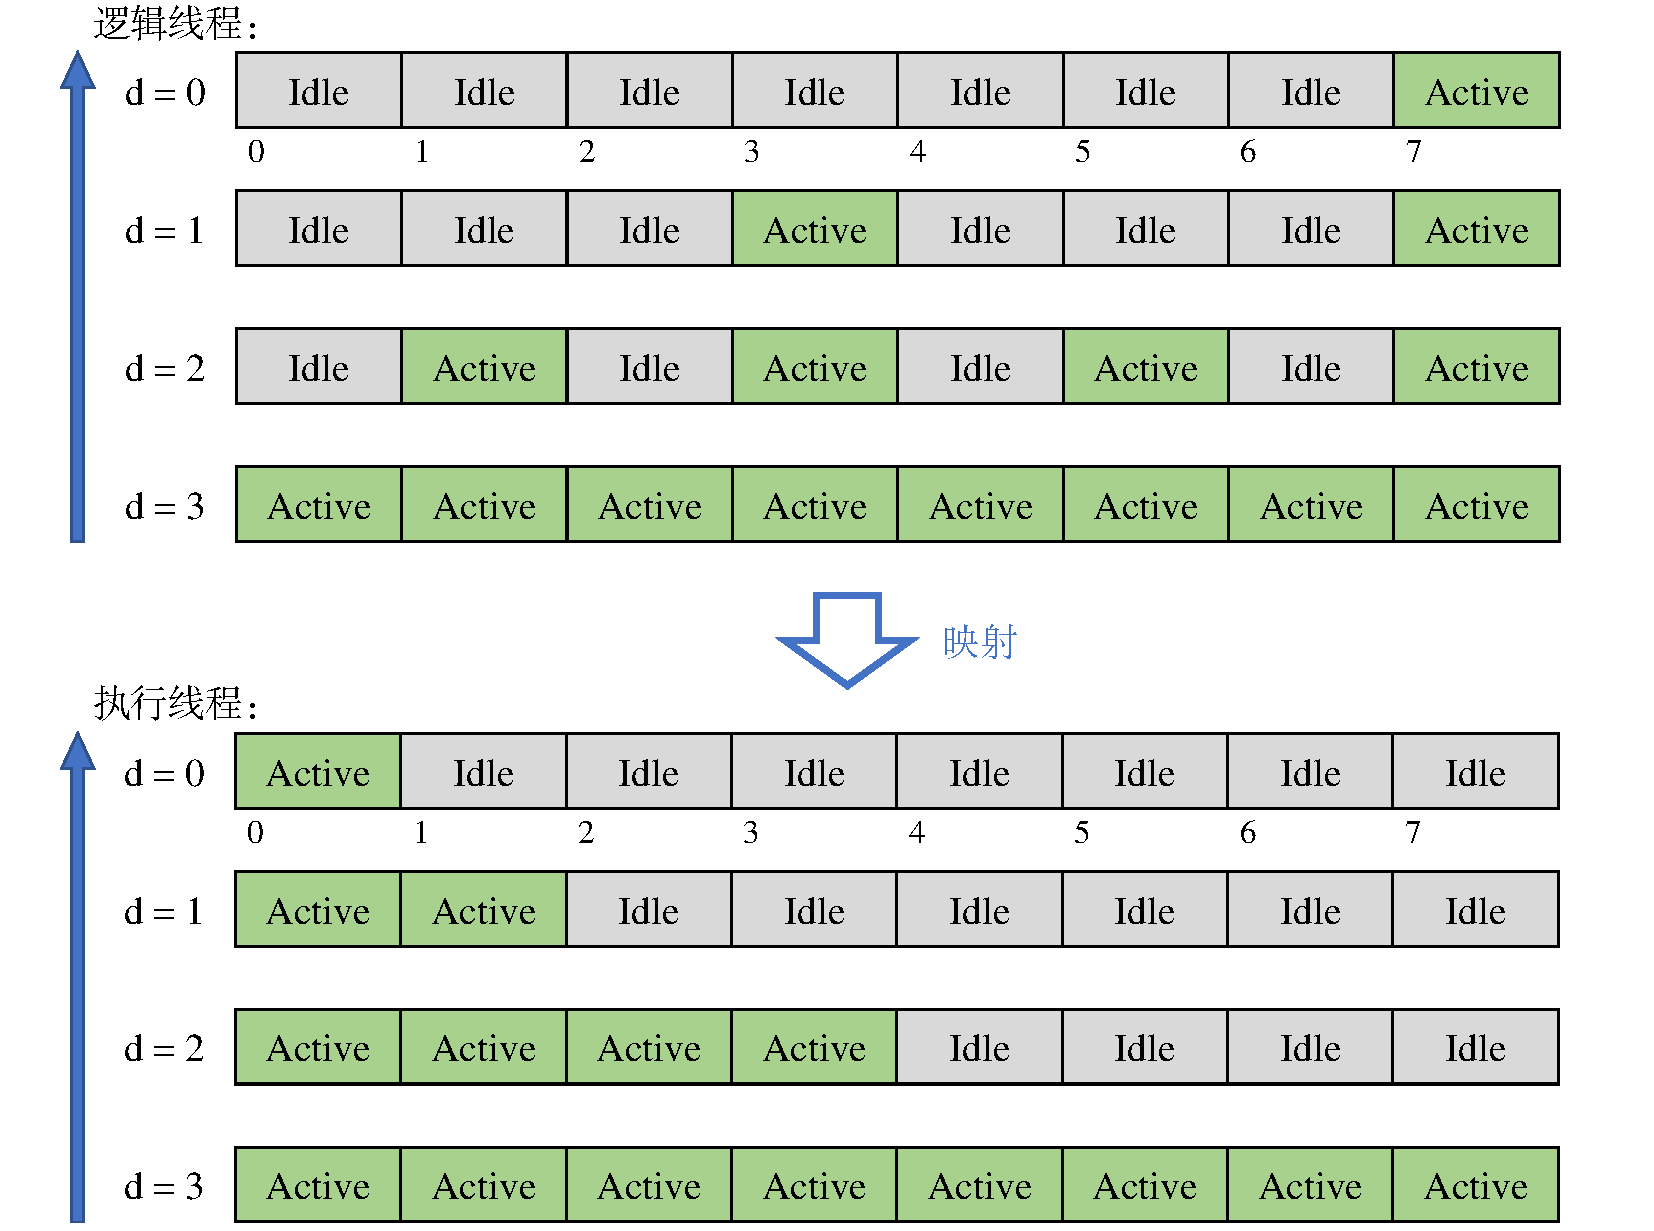
\includegraphics[width=.9\textwidth]{figures/neighbor/branch_divergence.pdf}
    	\caption{线程分支重映射}
    	\label{fig:remap}
    \end{figure}

\subsubsection{分支优化}
    GPU中包含大量计算单元,适合大量数据并行执行,但不适合执行分支指令。在英伟达的GPU架构中,一般32个流处理器组成一个warp。如果一个warp中线程执行的分支不同,则这一组线程就需要执行所有分支的指令,最后根据判断分支真假选择正确的结果,这显然会浪费大量计算资源。所以我们需要程序中连续的线程之间分支结果尽量相同,以减少分支分歧。
    
    但是在前缀和计算的向上以及向下扫描过程中,逻辑上的线程分支显然是不连续的(如图\ref{fig:upsweep}与\ref{fig:downsweep}),所以我们需要增加一层线程索引的映射(如图\ref{fig:remap}),从而使实际执行的线程分歧是连续的。
    
    \begin{figure}
    	\centering
    	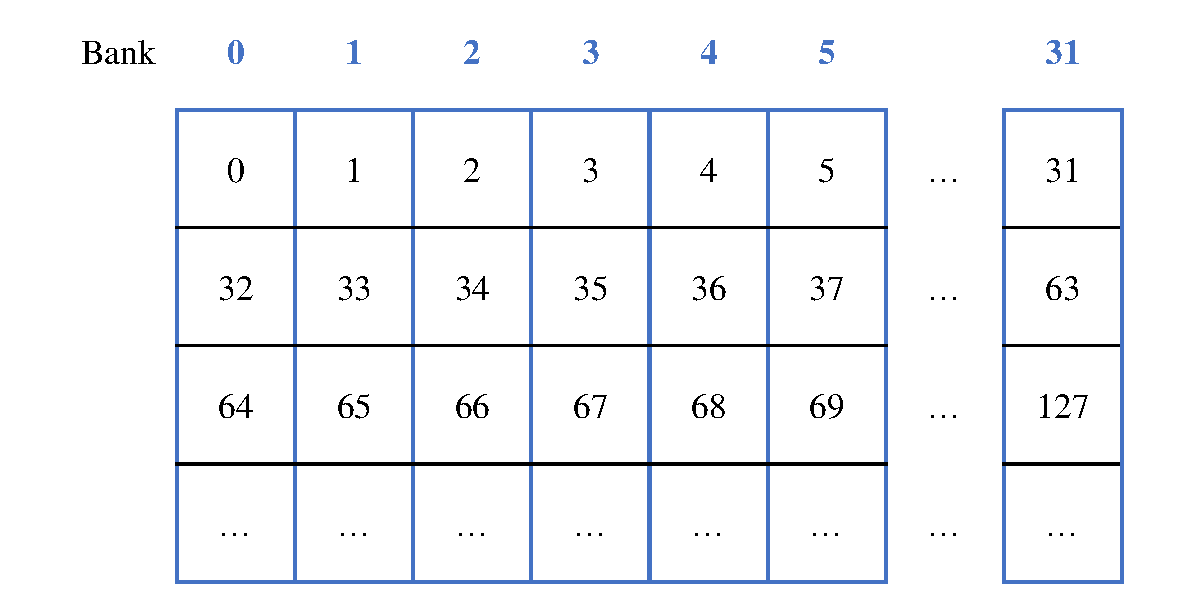
\includegraphics[width=.65\textwidth]{figures/neighbor/bank_conflict.pdf}
    	\caption{共享内存Bank}
    	\label{fig:bank}
    \end{figure}

\subsubsection{避免Bank冲突}
    为了实现共享内存高带宽的并行访问,共享内存被划分成了32个可以同时访问的等大小内存块(Banks,如图\ref{fig:bank}),且每4个字节被分配到了一个Bank中,每个Bank在一个时钟周期的带宽也为4字节。所以在读取共享内存时,如果访问不同Bank中的数据,则不会造成冲突;如果访问同一Bank中的同一个数据,则由于GPU的广播机制,也不会造成冲突;如果访问同一Bank中的不同数据,则由于带宽不足,会发生访存冲突(Bank Conflict),造成线程之间互相等待,使得并行计算退化为串行。
    
    在前缀和计算过程中,每次线程并行执行时访存地址间隔为2的指数倍,会造成Bank冲突。解决方法也很直接,在每32个数据间插入数量不等的空位,打乱访存地址,从而避免Bank冲突。
    
    \begin{figure}
    	\centering
    	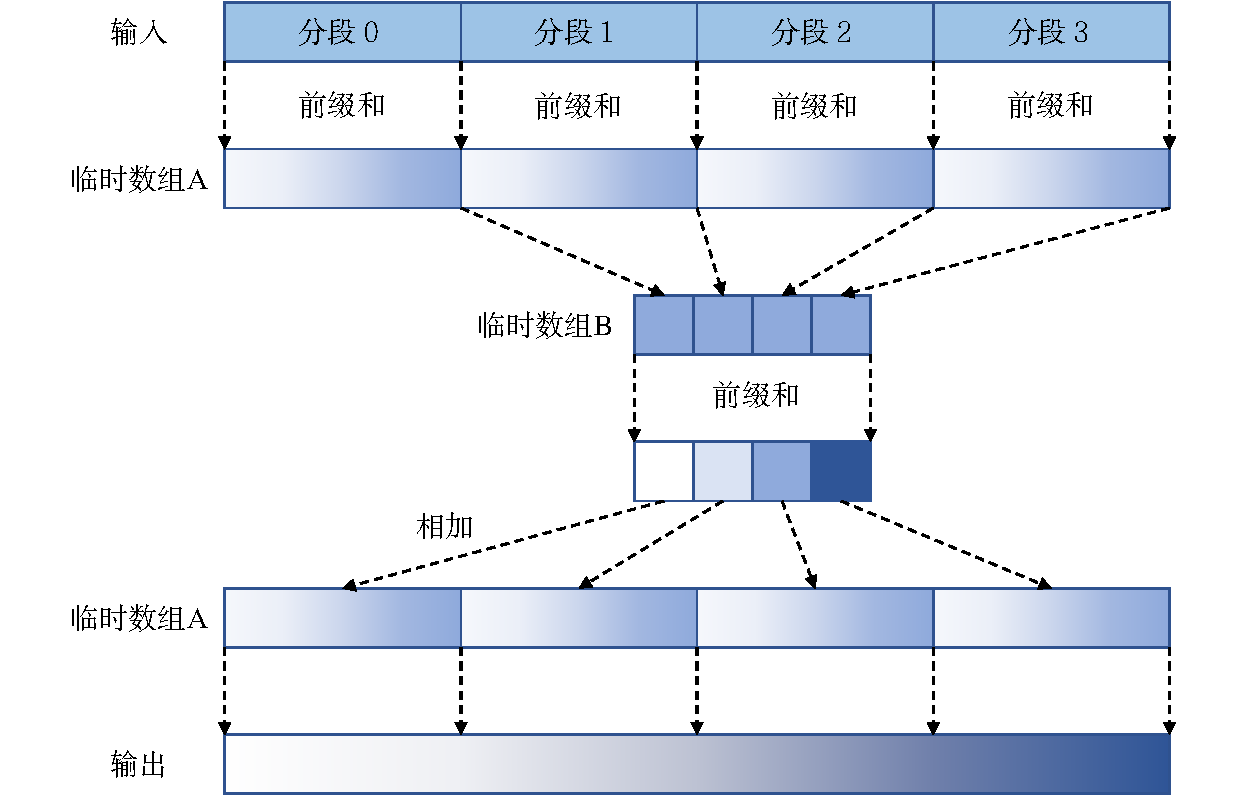
\includegraphics[width=.7\textwidth]{figures/neighbor/big_size_scan.pdf}
    	\caption{递归计算大数组前缀和}
    	\label{fig:bigarryscan}
    \end{figure}

\subsubsection{大数组前缀和}
    前文介绍的数组前缀和计算方法,都建立在同一个线程组的前提下,这是因为共享内存和线程同步指令都只能作用于相同的线程组。而由于WebGPU的限制,同一线程组最高支持256个线程(CUDA中最高支持1024个线程),这意味着我们只能计算最大长度位512的数组前缀和(每个线程读取两个数组元素),这显然是不够的。我们可以使用“递归”的思想解决这个问题(如图\ref{fig:bigarryscan}),对大数组以512长度分段,分别在每段内计算前缀和,再提取每段最后一个元素构成新数组,计算其前缀和,最后将结果加回对应段内的每一个元素。经过一次“递归”后,我们前缀和算法支持的数组最大长度为 $512\times512=2^{18}$(256k)。因此,我们的流体仿真系统最高支持将空间划分为256k个网格,同理,最大流体粒子数量也为256k。


\subsection{本章小结}
    本章详细阐述了邻域粒子并行搜索算法。其主要思想是空间在划分均匀网格来加速搜索,无论是寻找网格粒子,还是构建邻域粒子集,都使用了集合数组这一数据结构。在存储方式上,本章采用了不定长格式的存储结构,降低了存储消耗且增强了算法空间局部性。在其构建方法上,本章使用了计数排序的算法。另外,本章详细介绍了如何数组前缀和算法,他是实现计算排序的核心。尽管这一算法在逻辑上简单明了,但是由于其计算时数据间相互存在依赖,所以使用GPU高效并行化并不容易。最后,本章结合GPU硬件架构(如图\ref{fig:turing}),分别给出了在访存、分支与Bank冲突三方面的算法优化方案。
\clearpage
\section{实时流体渲染算法}
    本文中流体模拟的结果是粒子集,如果直接进行渲染,势必会得到凹凸不平的流体表面,真实感会大大下降。如果是离线渲染,可以使用移动立方体方法\cite{LC87MC}重建流体表面的高精度三角网格,再进行着色。显然这种方法不适用于实时渲染,所以本章设计了一套基于屏幕空间的动态流体渲染解决方案,在性能和资源受限的浏览器环境仍能高效渲染出可以接受的流体效果。

    \begin{figure}[htbp]
    	\centering
    	\includegraphics[width=.9\textwidth]{figures/rendering/raw_filterd.png}
    	\caption{流体粒子仿真结果与流体渲染效果}
    \end{figure}

\subsection{方法概述}
    屏幕空间方法法是实时渲染中的常用的一类方法,比如延迟渲染(Deffered Shading)、屏幕空间环境光遮蔽(Screen-Space Ambient Occlusion)、屏幕空间反射(Screen-Space Reflection)等。它指的是将场景光栅化之后,得到屏幕空间每个像素的几何与材质信息(法向、深度、反照率等),并将它们保存在多个帧缓冲之中(G-Buffer),再利用这些数据进行着色或其他光照计算。屏幕空间方法的复杂度仅与帧缓冲的分辨率有关,与场景复杂度无关,这使得它非常高效,并且适用于各种渲染管线。
    
    本章的流体渲染方案也以屏幕空间方法为基础\cite{G10SSF},首先将粒子实例化渲染,得到两张帧缓冲,分别保存流体表面深度与流体厚度,再对深度图进行平滑,最后进行光线着色。

\subsection{粒子实例化渲染}
    对于单个粒子,本章将其作为广告牌(Billboard)\cite{AHH19RTR}对象进行渲染。所谓广告牌就是固定朝向相机的贴图矩形。与球形网格相比,广告牌仅需两个三角形就可以表示一个粒子,大大减少了性能开销。同时,实验中利用硬件实例化技术渲染所有流体粒子,大大减少Drawcall数量,降低CPU与GPU通信开销。
    
    在着色器的具体实现上,首先根据uv值即可确定像素在矩形广告牌上的位置,如果在球体表面之外则直接丢弃,接下来计算流体表面的屏幕空间坐标,进而得到深度与厚度值。在计算深度图时,渲染管线开启深度测试。而在计算厚度图时,渲染管线关闭深度测试,并开启透明度混合,将着色器输出的厚度值利用硬件进行高效累加,得到每个像素对应流体的总厚度。

    \begin{figure}
    	\centering
    	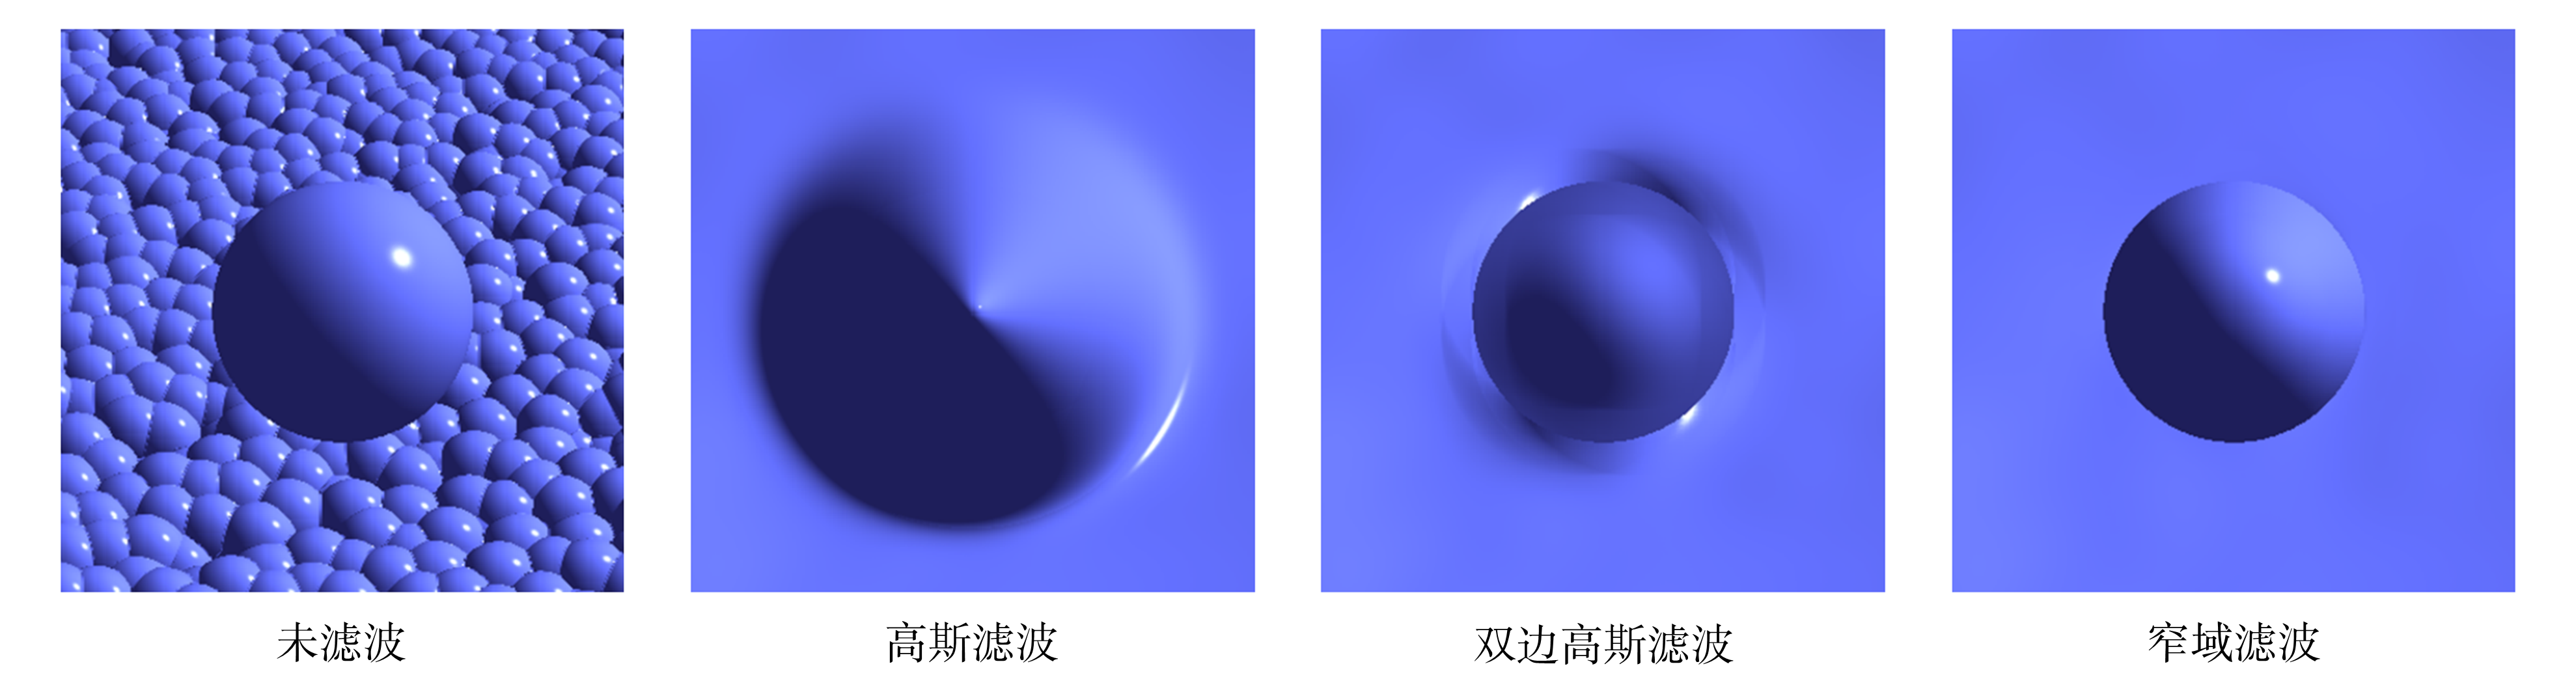
\includegraphics[width=.99\textwidth]{figures/rendering/filters.png}
    	\caption{不同滤波器滤波效果对比\cite{TY18NRSSF}}
    \end{figure}
    
    \begin{figure}
    	\centering
    	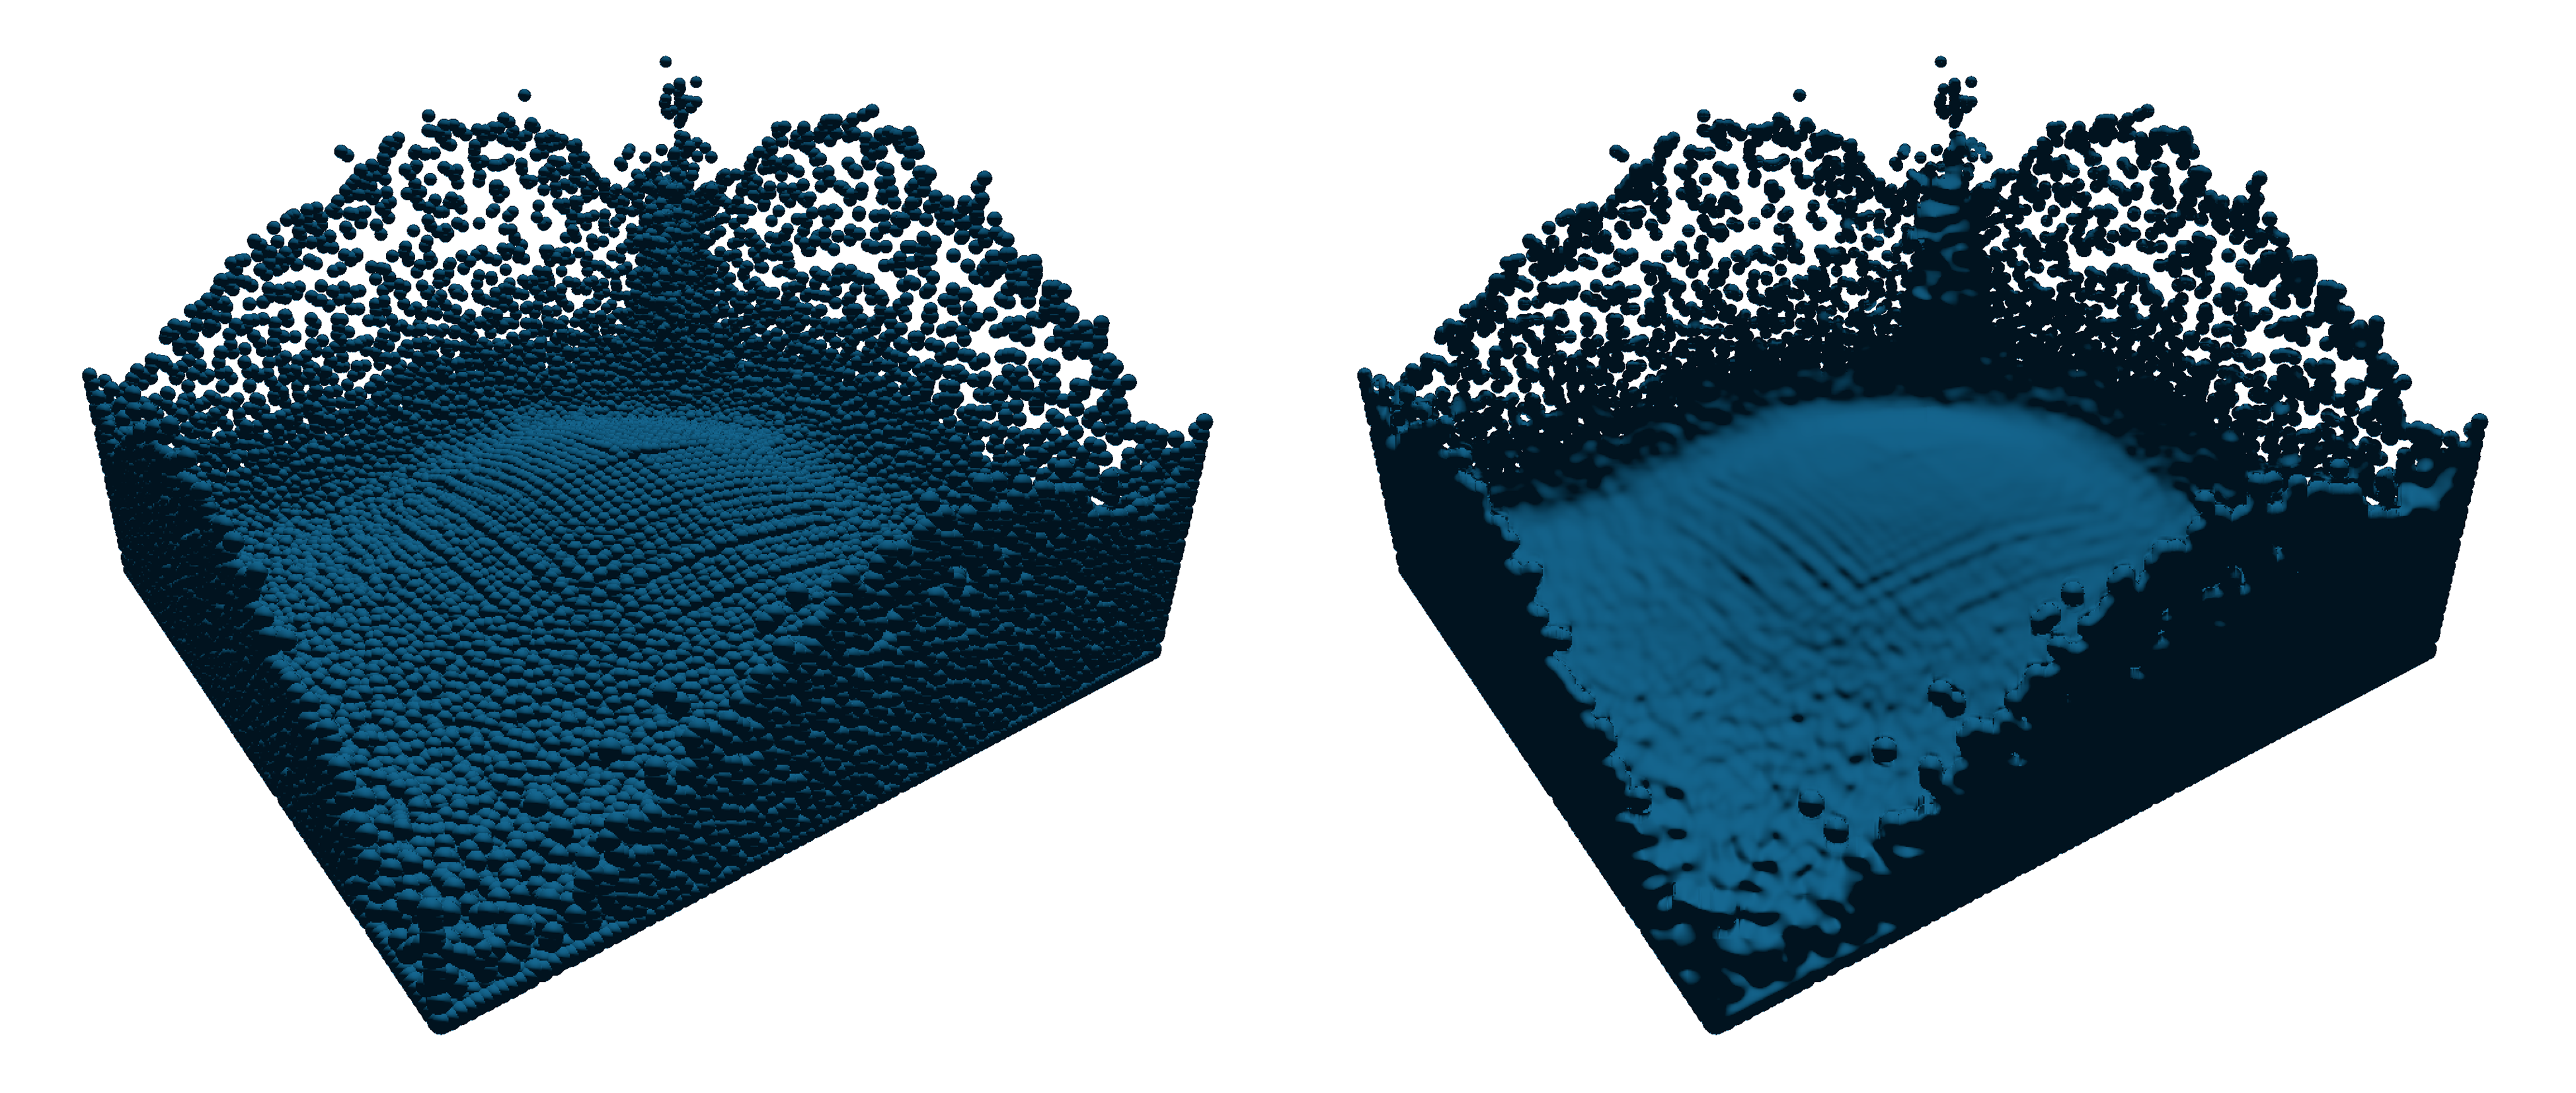
\includegraphics[width=.75\textwidth]{figures/rendering/before_after_filter.png}
    	\caption{深度滤波效果}
    \end{figure}

\subsection{深度图平滑}
    深度图平滑是提高流体渲染真实感的关键步骤。最直接的处理方式是高斯模糊,但这样会融合深度差异过大的表面,使得流体着色结果丢失轮廓边界。Green\cite{G10SSF}提出使用双边高斯滤波,能够有效保留表面轮廓,但是依然会导致边界附近深度值计算出现偏差。Truong等人\cite{TY18NRSSF}进一步提出了窄域滤波(Narrow-Range Filter),解决了双边滤波产生的问题。
    
    所谓窄域,指的是将待滤波的采样点深度值约束在一定范围内,减少深度差异过大的采样点影响滤波结果。窄域滤波的定义为
    \begin{equation}
    	z_i' = \frac {\sum_j \omega_{ij} f(z_i, z_j)}{\sum_j \omega_{ij}}
    \end{equation}
    其中 $z$ 为深度值,具体指的是相机坐标系下的线性深度(负值,即值越小越远离相机)。$z_i$ 为滤波中心采样点的深度值,$z_j$ 为其他采样点的深度值。$\omega_{ij}$ 为滤波权重,$f$ 为夹钳函数,其定义为
    \begin{equation}
    	f(z_i, z_j) = 
    	\left\{
    	\begin{array}{ll}
    	z_i - \mu, 	& \mathrm{if} \ z_j < z_i - \delta \\
    	z_j,   		& \mathrm{otherwise} \\
    	\end{array}
    	\right.
    \end{equation}
    其中 $\delta$ 定义的窄域的范围,$\mu$ 为用户指定的偏移量。此函数在允许的窄域范围内会返回原本的深度值 $z_j$,在采样点深度过深时会返回一个边界值 $z_i-\mu$ 。
    
    滤波权重的定义为
    \begin{equation}
    	\omega_{ij} =
    	\left\{
    	\begin{array}{ll}
    	0, 											& \mathrm{if} \ z_j > z_i + \delta \\
    	G(\mathbf{u}_i, \mathbf{u}_j, \sigma_i),   	& \mathrm{otherwise} \\
    	\end{array}
    	\right.
    \end{equation}
    其中 $\mathbf{u}_i$ 和 $\mathbf{u}_j$ 为采样点的位置坐标。$G$ 为高斯函数,$\sigma_i$ 为标准差,即
    \begin{equation}
    	G(\mathbf{u}_i, \mathbf{u}_j, \sigma_i) = \exp (\frac {-|\mathbf{u}_i - \mathbf{u}_j|^2} {2\sigma_i^2})
    \end{equation}
    
    \begin{figure}
    	\centering
    	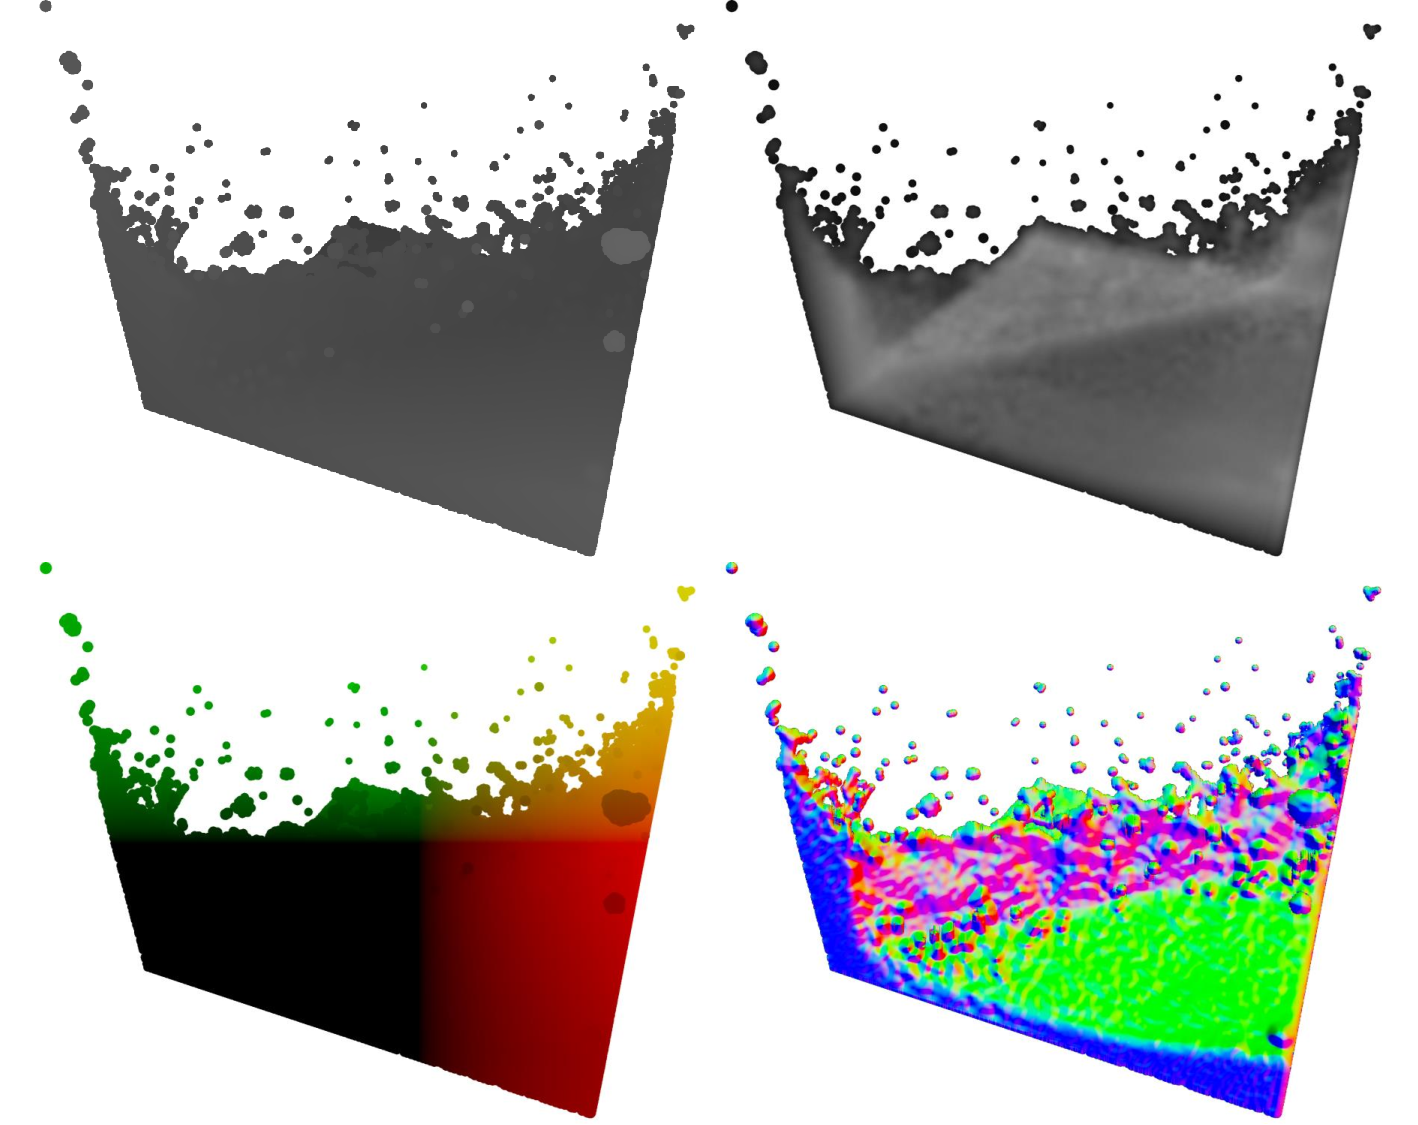
\includegraphics[width=.8\textwidth]{figures/rendering/d_t_p_n.pdf}
    	\caption{深度图(左上)厚度图(右上)位置还原效果(左下)法向还原效果(右下)}
        \label{fig:dtpn}
    \end{figure}
    
    综合公式6-3与公式6-4,采样点深度值在窄域范围内时滤波核权重与高斯核相同,但是在深度过浅时会将其贡献忽略调。但是直接忽略采样值会导致滤波核不对称,在流体表面法向与视线方向相差角度越大时,计算偏差越明显。为了解决这一问题,可以将深度过浅的采样点 $j$ 的对称位置 $k$ 的深度贡献同时忽略($\mathbf{u}_k = 2\mathbf{u}_i - \mathbf{u}_j$),以保证滤波核的对称性,调整之后滤波核的定义为
    \begin{equation}
    	\omega_{ij} =
    	\left\{
    	\begin{array}{ll}
    	0, 											& \mathrm{if} \ z_j > z_i + \delta \ \mathrm{or} \ z_k > z_i + \delta \\
    	G(\mathbf{u}_i, \mathbf{u}_j, \sigma_i),   	& \mathrm{otherwise} \\
    	\end{array}
    	\right.
    \end{equation}
    
    根据公式6-2与公式6-3,可以得到窄域范围的定义为 $z_i + \delta \ge z_j \ge z_i - \delta$。全局所有滤波点均使用这一窄域范围,显然这样定义是不准确的,因为流体表面深度的变化率差异较大,所以需要针对每个滤波点调整窄域范围。具体来说,可以在滤波过程中迭代调整窄域范围,设迭代过程中窄域定义为 $z_i + \delta_{high} \ge z_j \ge z_i - \delta_{low}$,其迭代初始值均设为 $\delta$,迭代策略为
    \begin{equation}
    	\begin{gathered}
    	\delta_{high} \leftarrow \max (\delta_{low}, z_i - z_j + \delta) \\
    	\delta_{low} \leftarrow \max (\delta_{low}, z_j - z_i + \delta)
    	\end{gathered}
    \end{equation}
    
    在具体实现上,由于2D滤波的效率在实时渲染中的计算量是不可接受的,所以本文将其拆分为x方向和y方向的两个1D滤波,不过在数学上这并不等价,会在流体轮廓边缘处造成轻微瑕疵。1D滤波核宽度设置为32像素,$\sigma$ 为1/4滤波核宽度,$\delta$ 为5倍粒子半径,$\mu$ 等于粒子半径。
    
    \begin{figure}
    	\centering
    	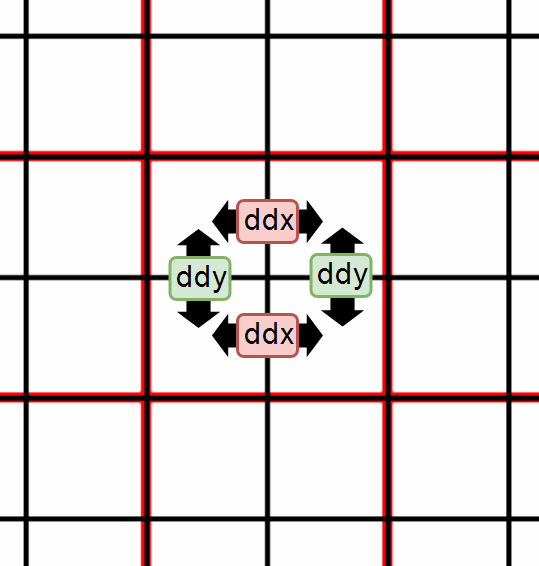
\includegraphics[width=.25\textwidth]{figures/rendering/ddx_ddy.png}
    	\caption{一阶差分}
    	\label{fig:difference}
    \end{figure}

\subsection{屏幕空间渲染}
    至此,得到平滑深度图与厚度图之后,就需要根据每个像素的深度、厚度、位置以及环境光信息完成着色。
    
    首先需要从深度 $z$ 与像素在平面上的位置 $[u,v]$ 还原其对应流体表面在相机坐标系下的位置坐标以及表面法向量。位置坐标可以很容易的通过像素位置与相机参数(屏幕分辨率 $[W, H]$,相机近平面距离 $n$)得到
    \begin{equation}
    	\mathbf{p} = z \
    	\left[
    	\frac{(u - 0.5) W} {n}, \;
    	\frac{(0.5 - v) H}{n}, \;
    	-1
    	\right]^T
    \end{equation}
    
    \begin{figure}
    	\centering
    	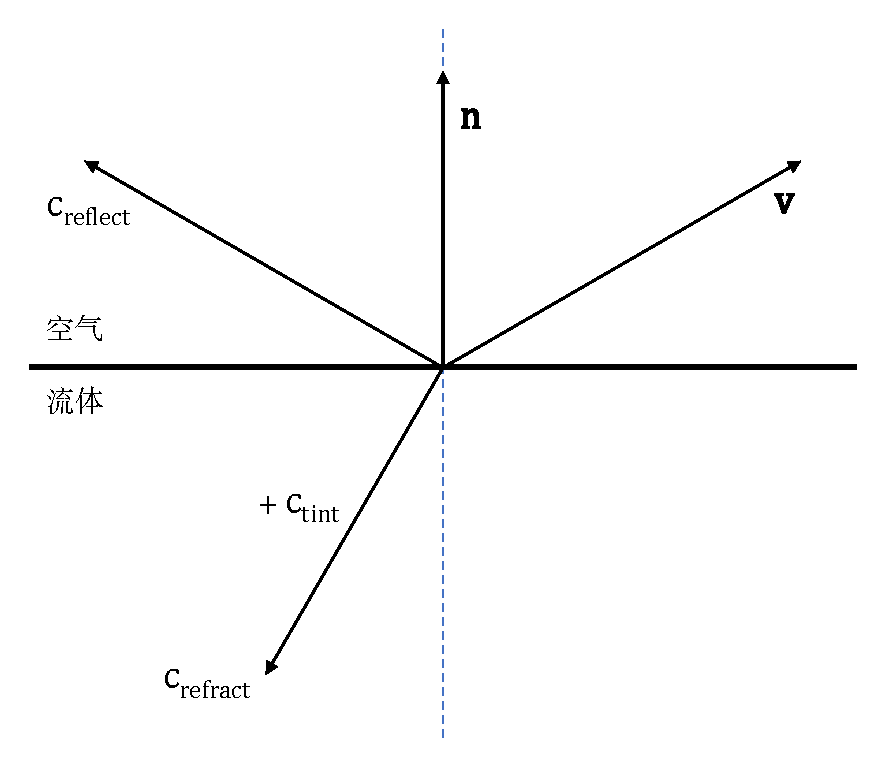
\includegraphics[width=.35\textwidth]{figures/rendering/shading.pdf}
    	\caption{反射与折射方向}
    	\label{fig:refraction}
    \end{figure}
    
    而法向可以看作流体表面两个不同的切线方向的叉乘,比如x方向和y方向。而切线又可以由流体表面位置的偏微分得到,所以法向的计算公式为
    \begin{equation}
    	\mathbf{n} = \frac {\partial \, \mathbf{p}} {\partial \, x} \times \frac {\partial \, \mathbf{p}} {\partial \, y}
    \end{equation}
    
    在硬件光栅化时,GPU往往会以 $2\times 2$ 的像素块为一个线程组进行计算,这样可以非常方便得在线程组内通过一阶差分近似偏微分(如图\ref{fig:difference})。同样,WebGPU在像素着色器中提供了偏微分内置函数dpdx()与dpdy(),所以我们可以非常容易地还原法向值,代码如下。

    \begin{listing}[htbp]
    \begin{minted}{glsl}
    fn getNormal(positionEye: vec3<f32>) -> vec3<f32> {
        let ddx = dpdx(positionEye);
        let ddy = dpdy(positionEye);
        let normalEye = normalize(cross(-ddx, ddy));
        return normalEye;
    }
    \end{minted}
    \caption{从深度图还原法向的wgsl着色器代码}
    \label{code:normal}
    \end{listing}
    
    在得到完整的几何信息之后,就可以进一步完成着色了。首先通过表面法向 $\mathbf{n}$ 和视线方向 $\mathbf{v}$ 计算菲涅尔项 $F$,它确定了在物体表面光线折射与反射的能量比值,本文采用了经典的Schick近似的菲涅尔计算公式\cite{S94BRDF}
    \begin{equation}
    	\begin{gathered}
    	F = F_0 + (1 - F_0) (1 - (\mathbf{n} \cdot \mathbf{v})^+)^5 
    	\\
    	F_0 = (\frac{n - 1}{n + 1})^2
    	\end{gathered}
    \end{equation}
    其中 $n$ 为物体表面折射率,代入水的折射率1.33可得 $F_0 \approx 0.02$ 。
    
    然后,我们可以根据反射和折射定律得到光线反射与折射方向,以这两个方向分别采样环境光贴图,即可得到流体表面的反射颜色 $c_{reflect}$ 与折射颜色 $c_{refract}$ 。折射颜色还需进一步与流体本征颜色 $c_{tint}$ 根据流体厚度衰减系数 $\gamma$ 进行插值(如图\ref{fig:refraction})。最后,以菲涅尔项 $F$ 确定反射颜色与折射颜色的比值,将其混合输出
    \begin{equation}
    	\begin{gathered}
    	c = \mathrm{lerp} ( \mathrm{lerp} (c_{tint},\ c_{refract},\ \gamma),\ c_{reflect},\ F ) 
    	\\
    	\gamma = exp(-t)
    	\end{gathered}
    \end{equation}
    
    \begin{figure}[htbp]
    	\centering
    	\includegraphics[width=.6\textwidth]{figures/rendering/result.png}
    	\caption{渲染结果}
    \end{figure}

\subsection{本章小结}
本章主要阐述了流体仿真系统的渲染部分的原理与实现。我们将物理模拟的结果——流体粒子,通过实例化渲染得到深度图与厚度图,再使用窄域滤波器平滑深度图,最后在屏幕空间完成流体渲染。相应地,在实现中我们使用WebGPU渲染-计算-渲染的混合管线架构,在实时物理模拟计算的同时完成高质量渲染,帧数几乎没有下降,这全面体现了WebGPU带来的新特性与性能优势。
\clearpage
\section{实时流体仿真系统的实现}
    本文的主要目标是基于WebGPU构建一个轻量级在线实时流体流体仿真系统。前文从物理模拟与流体渲染两个方面详细阐述了仿真系统的理论基础,本章将简要介绍WebGPU架构模型与API特性开始,并在此基础上进一步讨论流体模拟与渲染系统的具体实现,最后,本章使用流体仿真系统搭建了多个模拟场景,其实验结果全面体现了本文算法在轻量化、高效性与稳定性方面的优势,以及WebGPU广阔的应用场景。

    \begin{figure}[htbp]
    	\centering
    	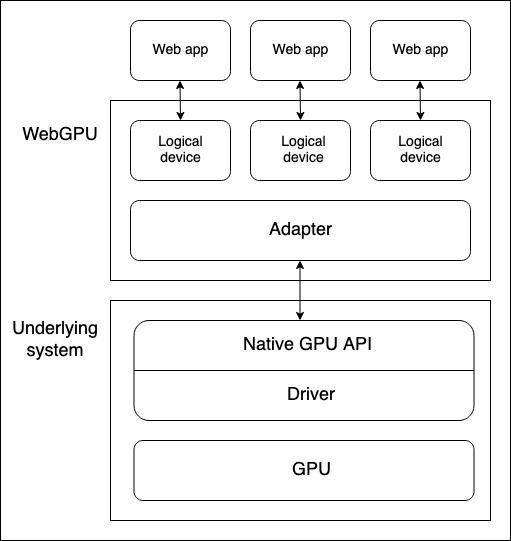
\includegraphics[width=.5\textwidth]{figures/webgpu/architecture.png}
    	\caption{WebGPU架构}
    \end{figure}

\subsection{WebGPU}
    WebGPU是一个全新的浏览器端图形API,它使开发人员能够使用底层系统的图形处理器(GPU)进行高性能计算并绘制可在浏览器中渲染的复杂图形。2023年5月,Chrome浏览器发布113版本,在稳定版中正式加入对WebGPU的支持。

    WebGPU并不是第一个浏览器图形API,2011年出现的WebGL是首个允许web页面直接将渲染计算传递给设备的GPU的图形接口。WebGL基于OpenGL设计实现,而自其发布之后,在原生平台又出现了新一代GPU API——微软的Direct3D 12、苹果的Metal以及Khronos组织的Vulkan,它们提供了大量新特性、更科学的设计与更高效的实现。这使得OpenGL逐渐落后于时代,同样WebGL也难以满足日新月异的浏览器应用的图形需求。因此,WebGPU应运而生,作为WebGL的继任者,它为现代GPU提供了更好的兼容性、支持更通用的GPU计算、更快的操作以及能够访问到更高级的GPU特性。
    
    WebGPU的设计更类似于Vulkan这类新一代GPU,摒弃了OpenGL全局状态机的管理模式。在与GPU交互时,WebGPU会先将所有指令都存储在指令队列(Commad Queue)中,一次性提交给GPU。一方面减少了CPU与GPU的通信损耗,另一方面在指令队列录制完毕后还可以多次使用,减少CPU冗余计算。最重要的WebGPU指令是设置绑定组(Bind Group)与管线(Pipeline)。绑定组描述了GPU计算时使用的存储资源的结构信息,而管线则确定了GPU如何计算,需要执行哪些着色器代码。后文将进一步介绍WebGPU支持的存储结构与管线配置。

    \begin{figure}
    	\centering
    	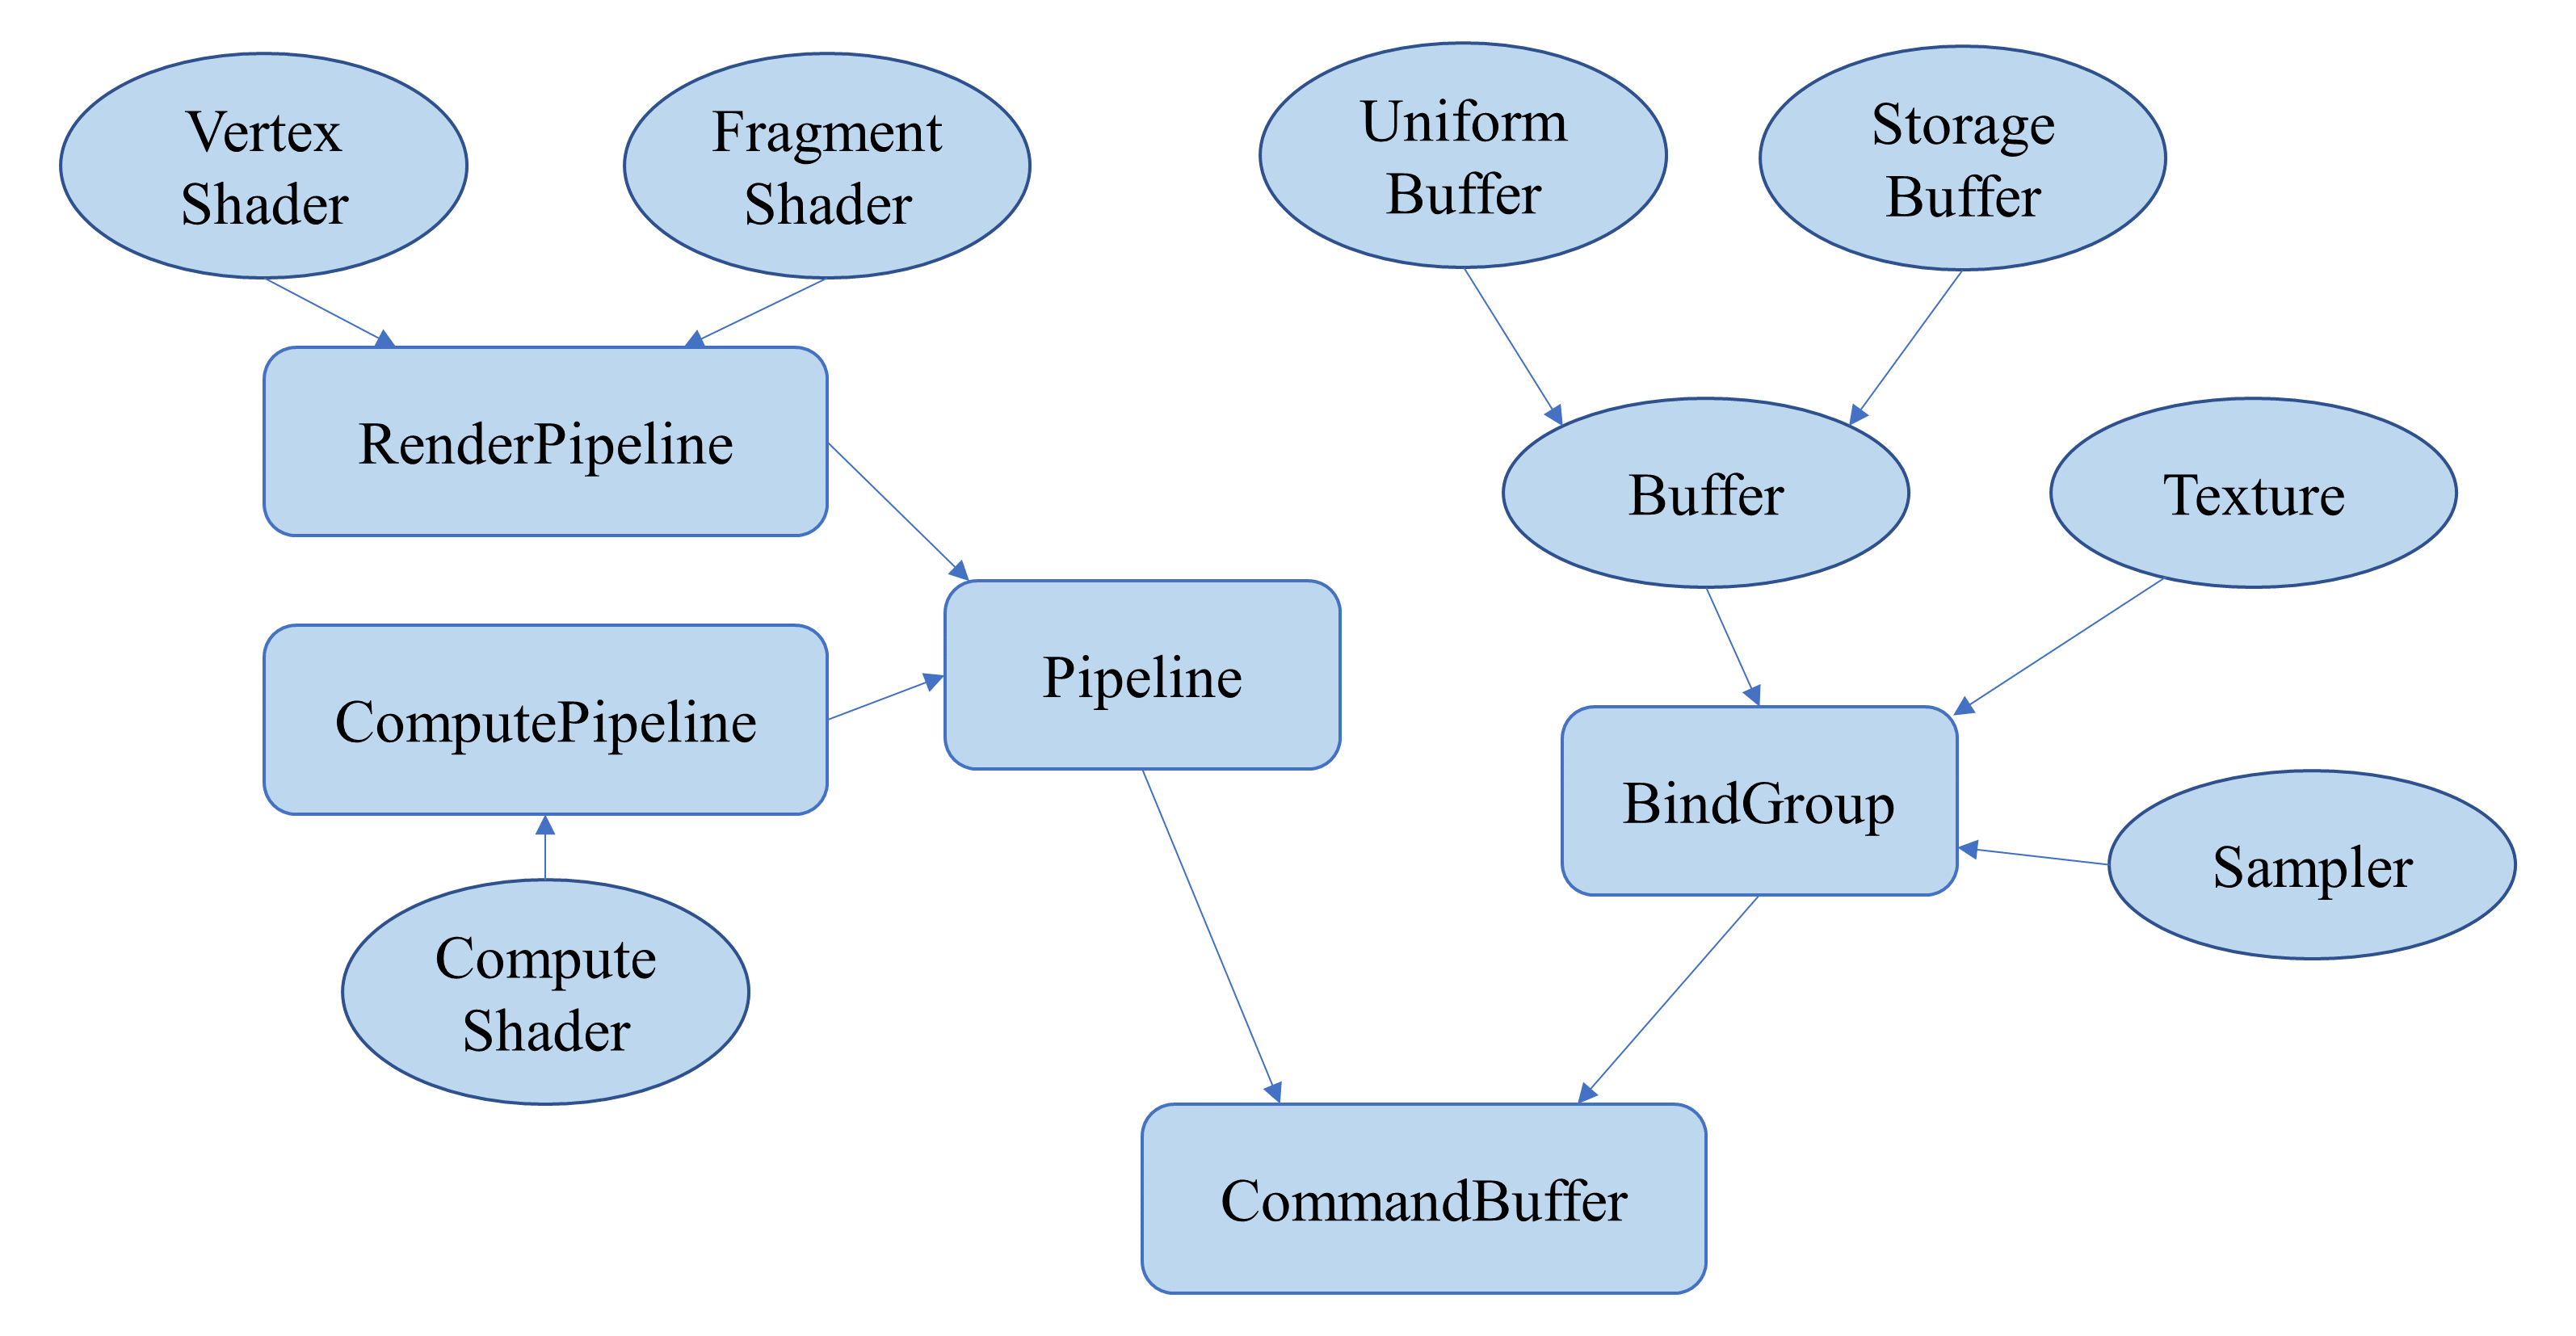
\includegraphics[width=.75\textwidth]{figures/webgpu/api.png}
    	\caption{WebGPU API结构}
    \end{figure}

\subsubsection{存储结构}
    WebGPU支持的存储类型有两种,Buffer与Texture。这两种存储结构以及采样器(Sampler)可以任意组合打包为绑定组,供计算管线与渲染管线使用。
    
    Buffer在存储中是线性结构,存储灵活自由。具体格式又分为两种:Uniform Buffer和Storage Buffer。其中Uniform Buffer是只读的,将数据传递到GPU后不可更改,在硬件上存储在常量内存区(Constant Memory),访问延迟较低。并且Uniform Buffer内存排布较为紧凑,需要以8字节为一块进行内存对齐,其空间最大为64KB。而Storage Buffer直接存储在显存上,可用空间非常大,但访问延迟也很高。
    
    基于以上特点,Uniform Buffer一般存储一些占用空间较小的,需要经常从CPU拷贝到GPU的常量信息,比如相机参数、光照信息、仿真参数、管线控制信息等。而Storage Buffer一般存储大量的,仅用于GPU计算的信息,比如仿真系统中每个粒子的物理量、空间网格结构、边界条件的体积贴图等。
    
    与Buffer不同,Texture在存储中是具有空间结构的,WebGPU支持1D/2D/3D纹理。在硬件结构上,Texture一般存储在专用的纹理内存中,访问速度较高,并且支持硬件的纹理采样、颜色空间转换等功能。另外,Texture对存储的数据结构有严格的要求,在创建时需要用户显示指定,比如rgba8unorm-srgb,意为4通道8位的纹理,其取值范围位0到1,并且数据精度为0-1均匀划分,另外在数据存储或读取时会自动做SRGB与线性之间的颜色空间转换。显然,Texture只用于纹理数据,或渲染管线输出的渲染目标(Render Target),例如流体渲染光栅化阶段的深度图与厚度图。

\subsubsection{管线}
    WebGPU管线分为两种,一个是传统的渲染管线(Render Pipeline),也就是GPU最基础的光栅化管线,另一个是计算管线(Compute Pipeline),它是WebGPU相对于WebGL引入的最重要新特性之一,它给开发者开放了GPU的通用计算能力,我们的流体仿真系统中绝大部分并行计算都依赖WebGPU计算管线实现。
    
    WebGPU渲染管线分为两个阶段(Stage),分别是顶点阶段和片元阶段,这两个阶段可以由开发者编写着色器程序进行自由控制。相比于其他现代图形API,WebGPU并不支持一些新型着色器,比如Tessellation Shader、Geometry Shader和Mesh Shader。这些着色器对应的阶段如顶点装配、光栅化、深度模板测试等直接由固定的硬件程序执行,开发者可以在管线创建时进行一些可选项的配置,比如图元拓扑结构、三角形剔除模式、alpha混合等。在仿真系统中,流体粒子的光栅化、流体屏幕空间渲染都使用渲染管线实现。
    
    WebGPU计算管线赋予了开发者极大的自由度,我们可以在计算着色器中读取Buffer或Texture中的数据,完成计算后将结果写入灵活的Storage Buffer中。在执行计算管线时可以指定任意数量个工作组(Work Group),并且工作组中的并行线程数量也可以在计算着色器中指定。并行计算往往会涉及到数据一致性的问题,WebGPU支持对同一存储空间进行原子读写操作,另外,同一工作组内的线程也可以在代码执行的任意位置进行线程同步。例如,在将数据读取到共享内存后,往往需要进行一次线程同步,以保证不同线程读取的数据均完成后再进行后续的计算操作。

\subsection{物理模拟系统}
    本文的目标是构建一个实时流体仿真系统,第三四五章分别介绍了流体模拟中的压强求解算法、非压强力算法与近邻粒子搜索算法。这些算法均具有高度的并行性,可以充分利用GPU算力优势。算法1给出了本系统的伪代码,其中所有for循环都是使用WebGPU的计算管线并行实现的,且每个for循环均对应一个计算着色器。由于本算法完全使用GPU并行化,所以不需要CPU与GPU之间的数据通信,这大大提高了计算效率。
    
    另外,本文也充分考虑了存储空间的优化。一个时间步之内,每个计算管线使用到的物理量不同,其中一些是完全互斥的,那么它们就可以重复使用同一块存储空间,比如在计算法向 $\mathbf n_i$ 时可以占用粒子位置 $\mathbf x_i^*$ 的存储空间。最终,在不影响数据对齐的前提下,每个粒子相关的物理量所占用的空间仅为84字节(32位浮点数精度)。

    \begin{algorithm}
    	\caption{流体仿真}
    	\begin{algorithmic}[1]
     
    	\ForAll{ particles $i$ } \Comment{ semi-implicit time integration }
    		\State apply force $\mathbf v_i \leftarrow \mathbf v_i + \Delta t \mathbf \, a_i$
    		\State predict position $\mathbf x^*_i \leftarrow  \mathbf x_i + \Delta t \mathbf \, v_i$
    	\EndFor

    	\ForAll{ particles $i$ } \Comment{ neighborhood particle search }
    		\State insert $\mathbf x^*_i$ into grid cell
    	\EndFor
    	\State calculate prefix sum of gridCellParticleCounts.
    	\ForAll{ particles $i$ } 
    		\State get sorted index of $\mathbf x^*_i$ \quad \Comment{ counting sort }
    	\EndFor
    	\ForAll{ particles $i$ } 
    		\State calculate count of neighboring particles of $\mathbf x^*_i$
    	\EndFor
    	\State calculate prefix sum of neighborParticleCounts.
    	\ForAll{ all particles $i$ } 
    		\State find neighboring particles $N_i(\mathbf x^*_i)$
    	\EndFor

    	\While { iter < iterCount } \Comment{ solve pressure constrain }
    		\ForAll{ particles $i$ }
    			\State calculate boundary volume $V_i^{\mathcal B}$ and boundary point $\mathbf x_i^*$  \quad \Comment{ Eq.\,3.15 }
    		\EndFor
    		\ForAll{ particles $i$ }
    			\State calculate $\lambda_i$  \quad \Comment{ Eqs.\,3.10,\,3.17 }
    		\EndFor
    		\ForAll{ particles $i$ }
    			\State calculate $\Delta \mathbf x_i$  \quad \Comment{ Eqs.\,3.12,\,3.19 }
    		\EndFor
    		\ForAll{ particles $i$ }
    			\State update predicted position $\mathbf x^*_i \leftarrow \mathbf x^*_i + \Delta \mathbf x_i$
    		\EndFor
    	\EndWhile
    	\ForAll{ particles $i$ }
    		\State update velocity $\mathbf v_i \leftarrow \frac{1}{\Delta t} (\mathbf x^*_i -\mathbf x_i)$
    		\State update position $\mathbf x_i \leftarrow \mathbf x^*_i$
    		\State update density $\rho_i = \sum_j m_j W_{ij}$
    	\EndFor

        \ForAll{ particles $i$ } \Comment{ apply non pressure forces }
            \State calculate normal $\mathbf n_i$  \quad \Comment{ Eq.\,4.4 }
            \State calculate vorticity $\omega_i$  \quad \Comment{ Eq.\,4.7 }
        \EndFor
        \ForAll{ particles $i$ }
            \State apply surface tension, vorticity confinement and XSPH \Comment{ Eqs.\,4.5,\,4.6,\,4.8 }
            \State calculate acceleration $\mathbf a_i \leftarrow \frac{\mathbf F_i}{m_i}$
        \EndFor
     
        \end{algorithmic}
    \end{algorithm}

\subsection{渲染系统}
    在实现了流体模拟系统之后,渲染系统需要将其实时渲染出来。本文第六章介绍了屏幕空间流体渲染算法,在WebGPU实现中,本文采用了渲染-计算-渲染的混合架构。首先使用两个渲染管线,借助硬件高效光栅化大量流体粒子,得到深度图和厚度图。然后使用两个计算管线,分别对深度图进行X方向和Y方向的窄域滤波。最后再使用一个渲染管线完成着色并输出到屏幕上。

    \begin{figure}
    	\centering
    	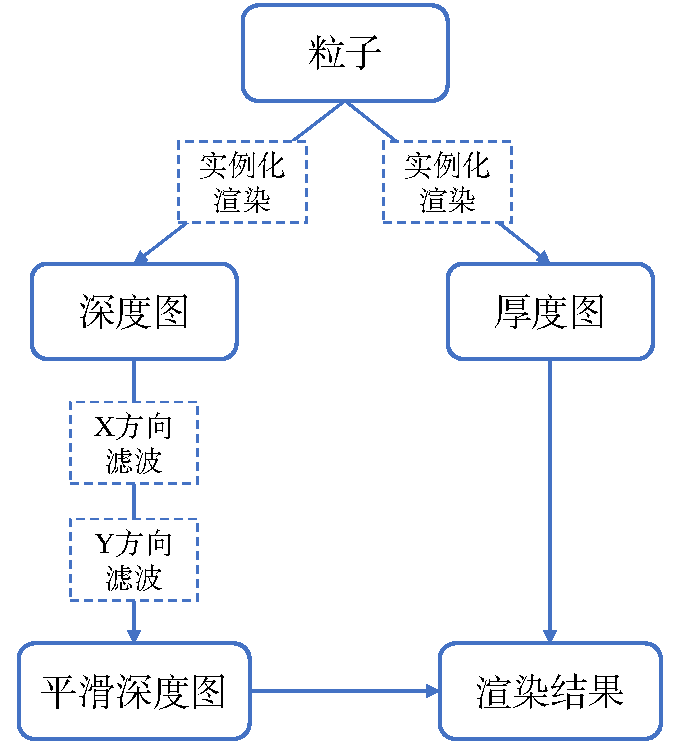
\includegraphics[width=.45\textwidth]{figures/webgpu/pipeline.pdf}
    	\caption{屏幕空间流体渲染流程图}
    \end{figure}

\subsection{实际仿真场景与性能分析}
    在本文搭建的流体仿真系统中,可人为调整的参数设置如下:仿真时间步长 $\Delta t = 0.005s$,密度约束中的松弛因子 $\varepsilon = 10^{-6}$,密度约束迭代次数为5次,表面张力 $\alpha = 0.5$,人工粘性 $\beta=0.01$,涡量补偿$\gamma = 0.1$。

    \begin{table}
    	\centering
    	\caption{帧率对比}
    	\begin{tabular}{ccc}
    	\toprule
    	实验场景 & 粒子数量(个) & 平均帧率(FPS) \\
    	\midrule
    	体素化兔子 & 32522	& 58.18	\\
    	立方体 & 68921	& 33.94	\\
    	水滴	 & 44489 & 45.07	\\
    	双溃坝 & 56448	& 27.08	\\
    	圆环边界 & 68921	& 22.88	\\
    	\bottomrule
    	\end{tabular}
    \end{table}
    
    \begin{table}
    	\centering
    	\caption{计算耗时对比}
    	\begin{tabular}{ccccccccc}
    	\toprule
    	\multirow{2}{*}{实验场景} &
    	\multicolumn{4}{c}{模拟} &
    	\multicolumn{4}{c}{渲染} \\
    	\cmidrule(lr){2-5} \cmidrule(lr){6-9}
    	& 时间积分 & 邻域查找 & 压强约束 & 非压强力 & 粒子光栅化 & 深度平滑 & 流体渲染 & 其他 \\
    	\midrule
    	体素化兔子
    	& 0.072	& 4.378	& 5.511	& 2.178	& 1.532	& 1.331	& 0.791	& 0.551	\\
    	立方体坠落
    	& 0.121	& 9.426	& 12.426& 4.871	& 2.718 & 1.364 & 0.848	& 0.547	\\
    	水滴			
    	& 0.094 & 5.822 & 8.092	& 3.451	& 2.034	& 1.385	& 0.742	& 0.578	\\
    	双溃坝		
    	& 0.104	& 12.070& 15.154& 6.077	& 3.117	& 1.697	& 0.989	& 0.672	\\
    	圆环边界		
    	& 0.121	& 14.949& 20.394& 7.452	& 3.808	& 1.780	& 1.080	& 0.707 \\
    	\bottomrule
    	\multicolumn{9}{r}{单位:毫秒}\\
    	\end{tabular}
    	\label{tab:comp}
    \end{table}
    
    图\ref{fig:result}展示了本仿真系统在五种不同实现场景下的模拟与渲染结果,从左到右分别是:体素化兔子、立方体、水滴、双溃坝与圆环边界,从上到下则表示了随着时间推移流体坠落的效果。其中兔子场景展示了本系统体素化控制流体初始边界的能力,水滴坠落展示了生动的流体表面张力效果,圆环边界展示了流体与固体交互的效果,立方体坠落与双溃坝则展示了本系统应对较大规模流体粒子的仿真效果。这五种复杂场景全面地体现了本系统的稳定性与模拟渲染的真实感。

    \begin{figure}
    	\centering
    	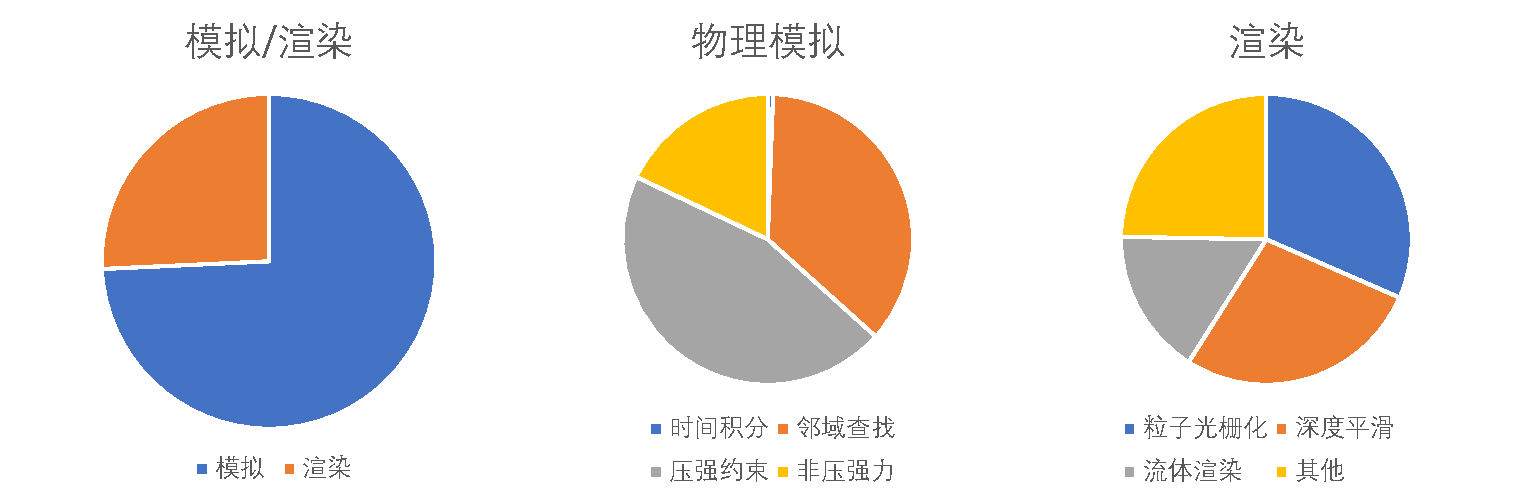
\includegraphics[width=0.9\textwidth]{figures/webgpu/comp.pdf}
    	\caption{计算耗时对比}
    	\label{fig:comp}
    \end{figure}
    
    \begin{figure}
    	\centering
    	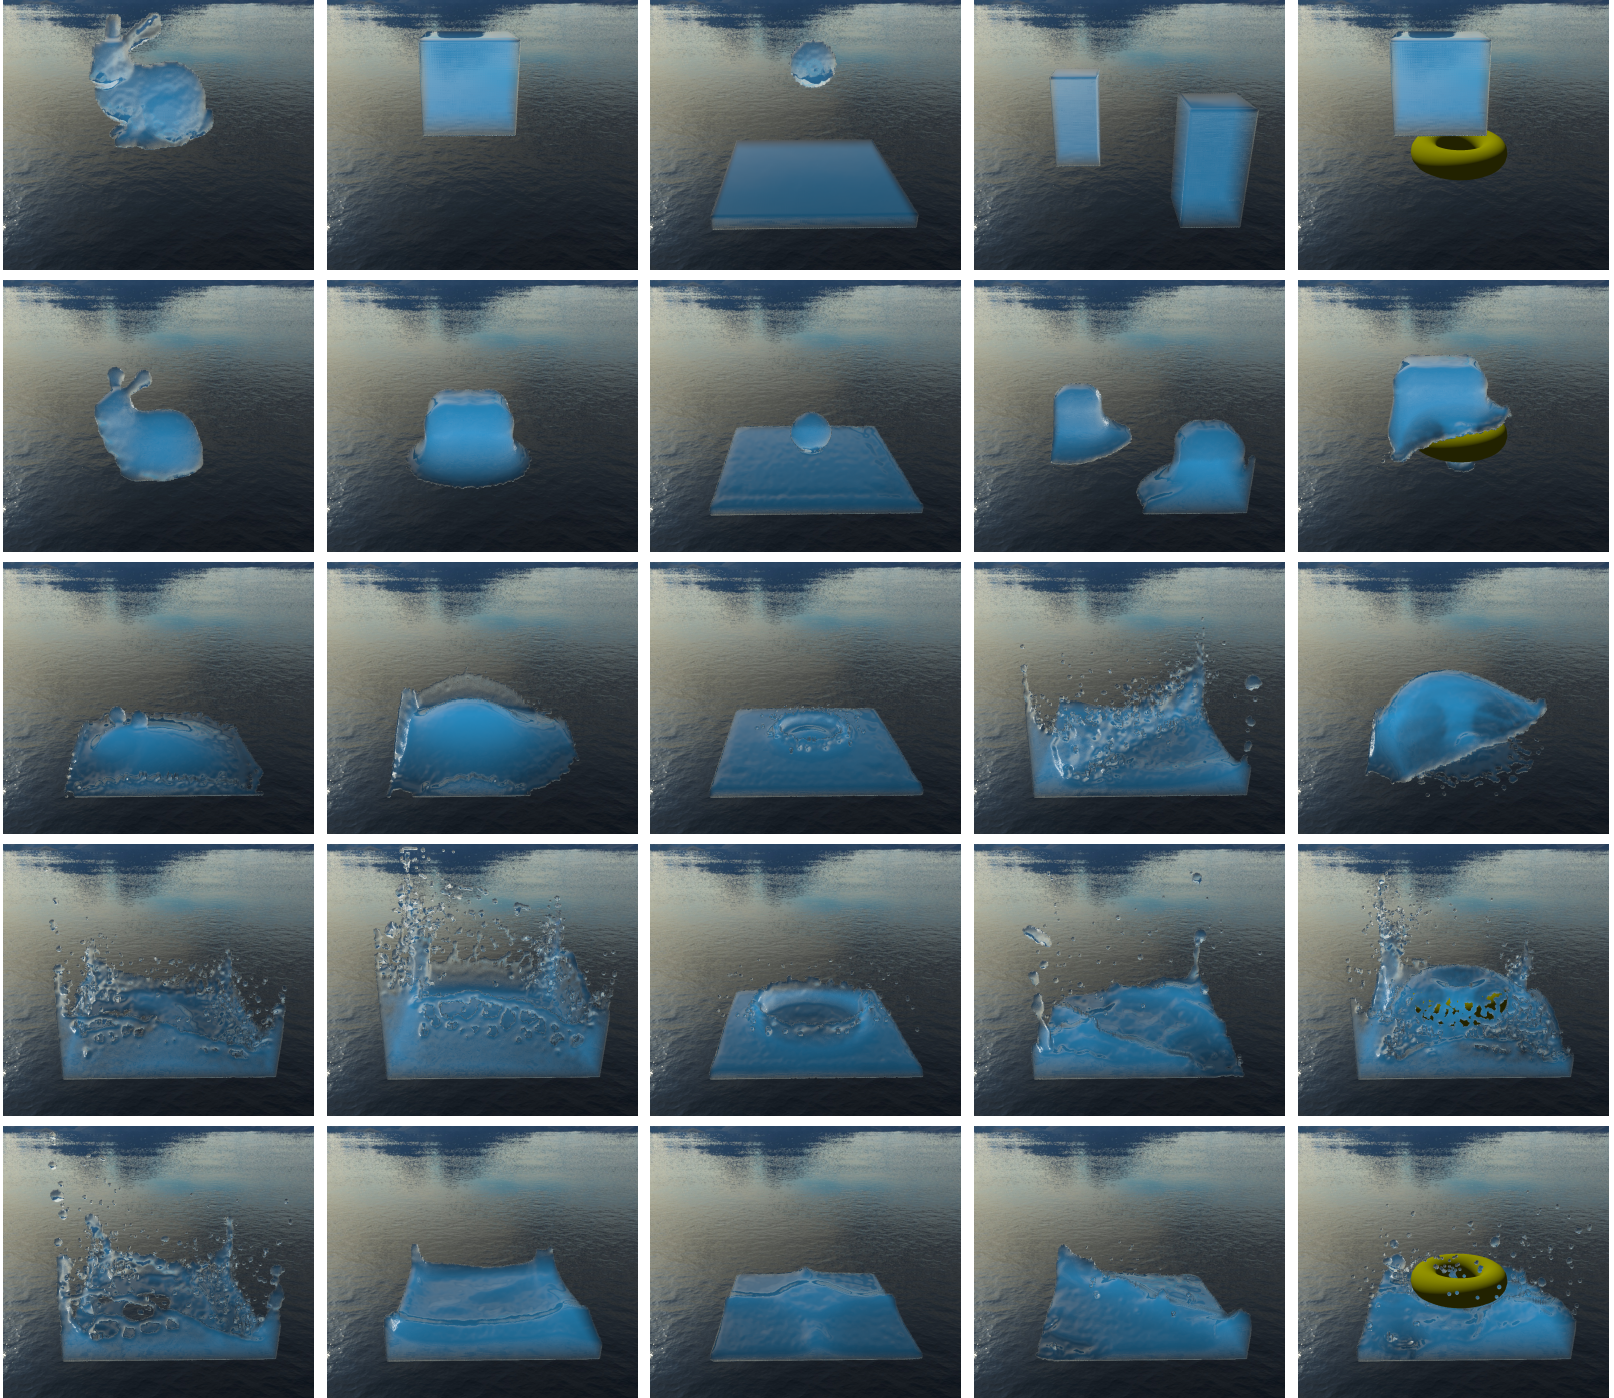
\includegraphics[width=0.99\textwidth]{figures/webgpu/demo.png}
    	\caption{实验结果(仿真场景:体素化兔子、立方体坠落、水滴、双溃坝与圆环边界)}
    	\label{fig:result}
    \end{figure}
    
    本章实验场景的测试平台硬件规格是:CPU为Intel Core i5-1135G7,RAM为16G,GPU为Intel Iris Xe(80EU)。本仿真系统仅运行在性能孱弱的集成显卡上,但仍然能够实时仿真并达到较流畅的30FPS,由此可见本文提出的轻量化流体仿真系统的高效性能。
    
    表\ref{tab:comp}与图\ref{fig:comp}给出了五个仿真场景前300帧每个模块计算的平均耗时。可以看出物理模拟计算耗时占每帧耗时的3/4,而这其中邻域粒子查找与压强约束求解又占了绝大部分时间。这点符合预期,因为邻域粒子查找数据相关性较强,其并行化算法较复杂,而压强约束需要迭代求解一个大型非线性系统,是整个仿真系统最耗时的计算模块。另外,由于我们将三种非压强力的实现压缩到了两个计算着色器中,这使得非压强力的计算耗时大大减少,远小于压强求解。在渲染计算方面,深度图的平滑是复杂度最高的计算过程,每个像素都需要采样大量相邻像素进行滤波计算,但由于我们在具体实现中使用了工作组线程间的共享缓存,大大减少了访存周期,使得深度平滑计算与硬件光栅化计算的耗时平分秋色。

\subsection{本章小结}
    本章阐述了实时流体仿真系统的实现。首先,本章从管线个存储结构两方面介绍了WebGPU的API架构,以及每种API在仿真系统的哪些模块中被使用到。其次,本章分别通过物理模拟模块的算法伪代码与流体渲染模块的流程图介绍了如何使用WebGPU实现仿真系统。最后,本章通过五个复杂场景证明了算法的稳定性与高效性,在核显平台仍然能达到实时仿真的帧率。总的来说,本文实现的流体仿真系统在实际应用中具有广阔的前景,可用于网页游戏、影视特效和虚拟现实等领域,提供更真实的交互和沉浸式体验。
\clearpage
\section{全文总结与展望}
\subsection{全文总结}
    本文提出并实现了一整套完整的基于粒子的流体模拟、渲染、交互系统。其中,流体模拟的关键在于保证不可压缩性求解流体压强,本文将基于位置的动力学(PBD)的思想应用于流体,推导出了基于位置的流体密度约束迭代求解方案。为了进一步完善边界处流体密度欠采样的问题,并实现固液耦合效果,本文采用了边界体积贴图(Volume Map)的隐式SPH边界处理方法。进一步,为了提高流体模拟的真实感,本文在流体压强求解器之后又加入了三种非压强力的求解模型。其次,在工程上,本文采用了空间网格划分加速邻域粒子搜索,并将其完全并行化。另外,本文又提出了一套针对粒子流体模拟结果的屏幕空间实时渲染方法。最后,本文将上述流体仿真方案整合为一套高度并行化的仿真算法,完全使用WebGPU实现。
    
    概况下来,本文的主要工作及贡献包括以下几点:
    
    \begin{enumerate}
    	\item 实现了基于位置的流体模拟方法。传统的SPH方法直接显式计算压强再通过时间积分更新粒子位置,仅能在时间步长很小的情况下才能保持稳定,这会变相降低流体模拟效率,难以应用在实时应用中。而基于位置的流体模拟方法同通过迭代计算密度约束的方法,保证了模拟过程中的流体不可压缩性,支持大时间步模拟。另外,相比于其他迭代求解方法,PBF直接更新粒子位置,没有采用传统的时间积分的方式,进一步简化了求解框架,使得其更适合应用于实时流体模拟。
    	\item 实现了隐式边界条件。粒子法在流体接近于固体边界的部分会由于欠采样而造成流体密度计算出现偏差,需要施加相应的边界条件实现流固耦合。传统的显示边界表示方式将固体边界体素化为粒子,并参与流体粒子的密度计算中。这种方式一方面会由于体素化的离散方式而产生较大误差。另一方面固体粒子也占用过多流体粒子的计算资源,在浏览器环境这种影响更加明显。而本文采用的边界体积方法是一种隐式边界表示方法,它需要将边界体积预计算为一张三维贴图,但是在流体模拟时可以快速查询边界条件对流体粒子的影响,在拥有更高计算精度的同时计算效率更高。
    	\item 通过添加非压强力改善流体细节。首先,由于在压强求解时我们没有考虑负压强的影响,所以本文在非压强力中添加了一个更加物理准确的表面张力模型。一方面在微观视角计算粒子内聚力,另一方面从宏观视角从表面曲率中计算最小化流体表面积的外力。其次,由于数值计算带来的阻尼,流体速度场涡量会快速降低,所以本文增加了一个涡量补偿力像系统中注入能量,保证流体的湍流细节。最后,由于压强解算使用的是密度约束而非速度散度约束,会造成流体速度场存在高频噪声,所以本文增加了人工粘性力,缓解粒子不真实的震荡现象。通过这三种非压强力,本文的流体模拟系统在实时仿真的同时能够保证足够的模拟真实感。
    	\item 实现了并行化的高效粒子搜索算法。临近粒子搜索往往是基于粒子的模拟方法的性能瓶颈。本文通过空间网格划分的方法加速了搜索算法的过程。但是算法中数据依赖性较强,本文使用了计算排序的方法,在不大量引入冗余存储空间的前提下使算法完全并行化。这其中一个重要算法是并行计算数组前缀和,本文采用了两趟遍历二叉树的思想使其并行化,并在具体实现中结合GPU硬件架构,在分支分歧、共享内存、内存Bank冲突等多方面进行优化,提高了粒子搜索的算法性能。
    	\item 实现了高效的屏幕空间流体渲染。在得到模拟结果流体粒子之后,传统的渲染方法往往是从大量粒子中提取表面网格,再将其通过传统的光栅化或光线追踪完成渲染,这在实时应用中显然是不可接受的。本文采用的渲染方法直接将这些流体粒子进行光栅化,不过并不是得到着色结果,而是得到深度和厚度图。然后使用窄域滤波器对深度图进行滤波,相比于双边滤波器,窄域滤波器能完全忽略深度差异过大的采用点之间的互相影响,在得到平滑的深度的同时保留流体边界的深度值突变。最后在屏幕空间完成流体渲染。这种渲染方法可以在保留流体真实感的同时高效执行。
    	\item 使用WebGPU在浏览器环境实现了本文介绍的流体仿真系统。传统的流体仿真由于性能要求,基本都使用C++在本地环境中构建,在跨平台、安装分享、硬件需求方面有着天然的劣势。但是随着新一代浏览器端图形API——WebGPU的发布,在浏览器端调用GPU资源运行流体仿真这种复杂应用遍成为了可能。本文使用了WebGPU实现了流体仿真系统,读者不需要安装任何插件即可浏览体现本流体仿真系统。 
    \\
    \href{https://linzhouli.github.io/WebGPU-Fluid-Simulation/}{https://linzhouli.github.io/WebGPU-Fluid-Simulation/}
    \end{enumerate}

    \begin{figure}[htbp]
    	\centering
    	\includegraphics[width=.9\textwidth]{figures/webgpu/result.png}
    	\caption{流体仿真系统}
    \end{figure}

\subsection{存在的不足}
    本文提出的流体仿真系统仍存在许多不足,概况如下:
    
    \begin{enumerate}
    	\item 流体模拟真实感欠佳。在流体压强解算方面,本文实现的PBF框架会仍会造成密度约束求解不充分,流体显得比较“粘滞”,能量耗散较快。在表面张力方面,流体会聚集成团状,难以形成真实的“藕断丝连”的效果,并且本文仅实现了流体粒子之间的内聚力,并没有实现流体与固体之间的黏着力,未能表现出疏水或亲水材质的效果。在流体粘性方面,本文仅采用了简单的显示处理方式,无法表现大粘度流体,比如蜂蜜,酸奶等。
    	\item 流体渲染中,深度图滤波后出现瑕疵。处于性能考虑。本文将深度平滑阶段使用的2D窄域滤波核拆分为两个1D滤波核,分别为X方向和Y方向,但是窄域滤波在数学上并不是可分离的滤波核,这样实现会造成流体轮廓处出现一定瑕疵,在法向还原后会更加严重(如图\ref{fig:dtpn})。这种现象可以通过在两个1D滤波后进行一次小的2D滤波来缓解,但本文并未实现。
    	\item 流体规模较小。由于WebGPU对工作组线程数量的限制,前缀和计算算法最高支持的数组长度也有上限,所以本仿真系统最高支持的流体粒子数量为256K个,相比于本地流体模拟百万级的粒子规模,本仿真系统在仿真细节上有一定缺失。
    	\item 不支持动态边界条件。本文实现的隐式边界条件处理方法仅支持静态物体边界,无法实现双向流固耦合,比如皮球漂浮在水面上随波逐流的效果。
    	\item 邻域粒子查找效率仍有待提高。文本实现的邻域粒子查找方法通过空间划分的结构进行加速,在排序时可以进一步使用网格的z-cureve索引,使得空间上靠近的粒子的物理信息在实际的线性存储空间内也相对靠近,可以大大提高算法的空间局部性,提高缓存命中率。
    \end{enumerate}

\subsection{未来展望}
    本文证明了使用WebGPU在浏览器环境中实现3D复杂流体实时仿真的可行性,并展示了浏览器端流体仿真的广阔应用场景和研究前景。
    
    首先,我们可以将更多高效的GPU并行物理模拟算法移植到浏览器环境中,以充分利用其跨平台优势。例如,布料仿真算法、毛发模拟算法、光线追踪算法等等。
    
    其次,WebGPU流体仿真可以应用于各种实际应用中,例如网页游戏、影视特效、WebVR等。通过实时的复杂3D流体模拟,这些应用可以获得更高的真实感和沉浸感,提升用户体验。
    
    最后,WebGPU为浏览器提供了更底层的GPU计算能力,为在浏览器中运行机器学习模型(WebML)提供更高效的支持。随着ChatGPT引发了下一轮AI热潮,浏览器端也出现了基于WebGPU的大规模模型,例如WebLLM和Web Stable Diffusion。此外,AI在科学领域的应用也正如火如荼,这些条件使得通过深度学习模型加速的Web端流体仿真成为可能。
    
    总之,WebGPU在浏览器端流体仿真的应用为各个领域带来了令人兴奋的可能性,涵盖了娱乐和科学研究等广泛范围。随着网络技术的不断发展和对真实感和交互性体验的需求不断增加,浏览器端流体仿真具备令人期待的未来发展前景。
\clearpage

\addcontentsline{toc}{section}{参考文献}
\bibliography{reference}

\clearpage
\section*{谢\ 辞}
\addcontentsline{toc}{section}{谢辞}

在完成本篇毕业论文期间,我要向所有支持和帮助过我的人表示衷心的感谢。

首先,我要感谢同济大学软件工程专业的教师们。感谢你们在教学过程中传授的知识和指导,为我提供了坚实的学术基础和专业素养。你们的教诲让我受益匪浅,为我的研究工作提供了重要的支持和指导。

此外,我要感谢同学们和朋友们。感谢你们在学习和研究过程中的帮助和支持。你们的讨论、交流和合作让我得以分享思想、解决问题,并激发了我进一步探索的动力。

我还要感谢我的家人。感谢你们对我学业的支持和理解。你们的鼓励和关心是我不断前进、克服困难的动力和支持。

\end{document}
